%===============================================================================
% LaTeX sjabloon voor de bachelorproef toegepaste informatica aan HOGENT
% Meer info op https://github.com/HoGentTIN/latex-hogent-report
%===============================================================================

\documentclass[dutch,dit,thesis]{hogentreport}

% TODO:
% - If necessary, replace the option `dit`' with your own department!
%   Valid entries are dbo, dbt, dgz, dit, dlo, dog, dsa, soa
% - If you write your thesis in English (remark: only possible after getting
%   explicit approval!), remove the option "dutch," or replace with "english".

\usepackage{lipsum} % For blind text, can be removed after adding actual content

%% Pictures to include in the text can be put in the graphics/ folder
\graphicspath{{graphics/}}

%% For source code highlighting, requires pygments to be installed
%% Compile with the -shell-escape flag!
\usepackage[section]{minted}
\usepackage[dutch,dutch]{babel} % Specify languages
\usepackage{iflang} % Required for \IfLanguageName

%% If you compile with the make_thesis.{bat,sh} script, use the following
%% import instead:
%% \usepackage[section,outputdir=../output]{minted}
\usemintedstyle{solarized-light}
\definecolor{bg}{RGB}{253,246,227} %% Set the background color of the codeframe

%% Change this line to edit the line numbering style:
\renewcommand{\theFancyVerbLine}{\ttfamily\scriptsize\arabic{FancyVerbLine}}

%% Macro definition to load external java source files with \javacode{filename}:
\newmintedfile[javacode]{java}{
    bgcolor=bg,
    fontfamily=tt,
    linenos=true,
    numberblanklines=true,
    numbersep=5pt,
    gobble=0,
    framesep=2mm,
    funcnamehighlighting=true,
    tabsize=4,
    obeytabs=false,
    breaklines=true,
    mathescape=false
    samepage=false,
    showspaces=false,
    showtabs =false,
    texcl=false,
}

% Other packages not already included can be imported here

%%---------- Document metadata -------------------------------------------------
% TODO: Replace this with your own information
\author{Yani Degrande}
\supervisor{Mevr. S. Vandermeersch}
\cosupervisor{Dhr. S. Braet}
\title[]%
    {Evaluatie van databaseoplossingen voor e-commerce in de mode-industrie: een focus op prestaties en kosten}
\academicyear{\advance\year by -1 \the\year--\advance\year by 1 \the\year}
\examperiod{1}
\degreesought{\IfLanguageName{dutch}{Professionele bachelor in de toegepaste informatica}{Bachelor of applied computer science}}
\partialthesis{false} %% To display 'in partial fulfilment'
%\institution{Internshipcompany BVBA.}

%% Add global exceptions to the hyphenation here
\hyphenation{back-slash}

%% The bibliography (style and settings are  found in hogentthesis.cls)
\addbibresource{bachproef.bib}            %% Bibliography file
\addbibresource{../voorstel/voorstel.bib} %% Bibliography research proposal
\defbibheading{bibempty}{}

%% Prevent empty pages for right-handed chapter starts in twoside mode
\renewcommand{\cleardoublepage}{\clearpage}

\renewcommand{\arraystretch}{1.2}

\usepackage{wrapfig}
\usepackage{graphicx}
\usepackage{hyperref}
\usepackage{listings}
\usepackage{booktabs}
\usepackage{pgfplots}
\pgfplotsset{compat=1.18}
\usepackage{array}
\usepackage{tabularx}
\usepackage{geometry}

%% Content starts here.
\begin{document}

%---------- Front matter -------------------------------------------------------

\frontmatter

\hypersetup{pageanchor=false} %% Disable page numbering references
%% Render a Dutch outer title page if the main language is English
\IfLanguageName{english}{%
    %% If necessary, information can be changed here
    \degreesought{Professionele Bachelor toegepaste informatica}%
    \begin{otherlanguage}{dutch}%
        \maketitle%
    \end{otherlanguage}%
}{}

%% Generates title page content
\maketitle
\hypersetup{pageanchor=true}

%%=============================================================================
%% Voorwoord
%%=============================================================================

\chapter*{\IfLanguageName{dutch}{Woord vooraf}{Preface}}%
\label{ch:voorwoord}

%% TODO:
%% Het voorwoord is het enige deel van de bachelorproef waar je vanuit je
%% eigen standpunt (``ik-vorm'') mag schrijven. Je kan hier bv. motiveren
%% waarom jij het onderwerp wil bespreken.
%% Vergeet ook niet te bedanken wie je geholpen/gesteund/... heeft

\lipsum[1-2]
%%=============================================================================
%% Samenvatting
%%=============================================================================

% TODO: De "abstract" of samenvatting is een kernachtige (~ 1 blz. voor een
% thesis) synthese van het document.
%
% Een goede abstract biedt een kernachtig antwoord op volgende vragen:
%
% 1. Waarover gaat de bachelorproef?
% 2. Waarom heb je er over geschreven?
% 3. Hoe heb je het onderzoek uitgevoerd?
% 4. Wat waren de resultaten? Wat blijkt uit je onderzoek?
% 5. Wat betekenen je resultaten? Wat is de relevantie voor het werkveld?
%
% Daarom bestaat een abstract uit volgende componenten:
%
% - inleiding + kaderen thema
% - probleemstelling
% - (centrale) onderzoeksvraag
% - onderzoeksdoelstelling
% - methodologie
% - resultaten (beperk tot de belangrijkste, relevant voor de onderzoeksvraag)
% - conclusies, aanbevelingen, beperkingen
%
% LET OP! Een samenvatting is GEEN voorwoord!

%%---------- Nederlandse samenvatting -----------------------------------------
%
% TODO: Als je je bachelorproef in het Engels schrijft, moet je eerst een
% Nederlandse samenvatting invoegen. Haal daarvoor onderstaande code uit
% commentaar.
% Wie zijn bachelorproef in het Nederlands schrijft, kan dit negeren, de inhoud
% wordt niet in het document ingevoegd.

\IfLanguageName{english}{%
\selectlanguage{dutch}
\chapter*{Samenvatting}

\selectlanguage{english}
}{}

%%---------- Samenvatting -----------------------------------------------------
% De samenvatting in de hoofdtaal van het document

\chapter*{\IfLanguageName{dutch}{Samenvatting}{Abstract}}

Tegenwoordig is er een exponentiële groei in het gebruik van e-commerce webshops. De onderliggende database speelt hierbij een belangrijke rol. Om developers binnen bedrijven in de toekomst te kunnen ondersteunen bij hun keuze voor een databaseoplossing, zal er een onderzoek gevoerd worden naar de meest geschikte database oplossing voor een e-commerce webshop in de mode-industrie. Het onderzoek richt zich op het evalueren van vijf verschillende database oplossingen. De focus zal hierbij gelegd worden op de prestaties en kosten van de desbetreffende databases. Het onderzoek zelf zal onderverdeeld worden in zes verschillende fases. In eerste instantie zal er een literatuurstudie worden gevoerd. In de stand van zaken zal informatie worden gegeven over de verschillende soorten databases die er bestaan en zal nagegaan worden welke databases momenteel gebruikt worden door het bedrijf Aware. Na de literatuurstudie volgt een requirements analyse waarin de functionele- en niet-functionele requirements voor dergelijk databasesysteem besproken worden. In een volgende stap wordt een short list van vijf verschillende databases opgesteld. Vervolgens wordt een vergelijkende studie van deze vijf databases uitgevoerd. Deze studie bestaat enkel uit gevonden literatuur en technische gegevens van deze databases. Nadien volgt een Proof of Concept (PoC) waarin elk van deze databases uitgetest wordt. In laatste instantie wordt op basis van de vergelijkende studie en de resultaten van de PoC een besluit getrokken die weergegeven wordt in de conclusie.

\vspace{5mm}

Op basis van dit onderzoek kunnen we besluiten dat de keuze van de database deels afhankelijk is van de voorkeuren van de developer. Indien geopteerd wordt voor een SQL databasesysteem wordt ClickHouse aangeraden. Indien de developer een voorkeur heeft voor een NoSQL database wordt vooral MongoDB aangeraden.

%---------- Inhoud, lijst figuren, ... -----------------------------------------

\tableofcontents

% In a list of figures, the complete caption will be included. To prevent this,
% ALWAYS add a short description in the caption!
%
%  \caption[short description]{elaborate description}
%
% If you do, only the short description will be used in the list of figures

\listoffigures

% If you included tables and/or source code listings, uncomment the appropriate
% lines.
\listoftables

\listoflistings



% Als je een lijst van afkortingen of termen wil toevoegen, dan hoort die
% hier thuis. Gebruik bijvoorbeeld de ``glossaries'' package.
% https://www.overleaf.com/learn/latex/Glossaries

%---------- Kern ---------------------------------------------------------------

\mainmatter{}

% De eerste hoofdstukken van een bachelorproef zijn meestal een inleiding op
% het onderwerp, literatuurstudie en verantwoording methodologie.
% Aarzel niet om een meer beschrijvende titel aan deze hoofdstukken te geven of
% om bijvoorbeeld de inleiding en/of stand van zaken over meerdere hoofdstukken
% te verspreiden!

%%=============================================================================
%% Inleiding
%%=============================================================================

\chapter{\IfLanguageName{dutch}{Inleiding}{Introduction}}%
\label{ch:inleiding}

De inleiding moet de lezer net genoeg informatie verschaffen om het onderwerp te begrijpen en in te zien waarom de onderzoeksvraag de moeite waard is om te onderzoeken. In de inleiding ga je literatuurverwijzingen beperken, zodat de tekst vlot leesbaar blijft. Je kan de inleiding verder onderverdelen in secties als dit de tekst verduidelijkt. Zaken die aan bod kunnen komen in de inleiding~\autocite{Pollefliet2011}:

\begin{itemize}
  \item context, achtergrond
  \item afbakenen van het onderwerp
  \item verantwoording van het onderwerp, methodologie
  \item probleemstelling
  \item onderzoeksdoelstelling
  \item onderzoeksvraag
  \item \ldots
\end{itemize}

\section{\IfLanguageName{dutch}{Probleemstelling}{Problem Statement}}%
\label{sec:probleemstelling}

Uit je probleemstelling moet duidelijk zijn dat je onderzoek een meerwaarde heeft voor een concrete doelgroep. De doelgroep moet goed gedefinieerd en afgelijnd zijn. Doelgroepen als ``bedrijven,'' ``KMO's'', systeembeheerders, enz.~zijn nog te vaag. Als je een lijstje kan maken van de personen/organisaties die een meerwaarde zullen vinden in deze bachelorproef (dit is eigenlijk je steekproefkader), dan is dat een indicatie dat de doelgroep goed gedefinieerd is. Dit kan een enkel bedrijf zijn of zelfs één persoon (je co-promotor/opdrachtgever).

\section{\IfLanguageName{dutch}{Onderzoeksvraag}{Research question}}%
\label{sec:onderzoeksvraag}

Wees zo concreet mogelijk bij het formuleren van je onderzoeksvraag. Een onderzoeksvraag is trouwens iets waar nog niemand op dit moment een antwoord heeft (voor zover je kan nagaan). Het opzoeken van bestaande informatie (bv. ``welke tools bestaan er voor deze toepassing?'') is dus geen onderzoeksvraag. Je kan de onderzoeksvraag verder specifiëren in deelvragen. Bv.~als je onderzoek gaat over performantiemetingen, dan 

\section{\IfLanguageName{dutch}{Onderzoeksdoelstelling}{Research objective}}%
\label{sec:onderzoeksdoelstelling}

Wat is het beoogde resultaat van je bachelorproef? Wat zijn de criteria voor succes? Beschrijf die zo concreet mogelijk. Gaat het bv.\ om een proof-of-concept, een prototype, een verslag met aanbevelingen, een vergelijkende studie, enz.

\section{\IfLanguageName{dutch}{Opzet van deze bachelorproef}{Structure of this bachelor thesis}}%
\label{sec:opzet-bachelorproef}

% Het is gebruikelijk aan het einde van de inleiding een overzicht te
% geven van de opbouw van de rest van de tekst. Deze sectie bevat al een aanzet
% die je kan aanvullen/aanpassen in functie van je eigen tekst.

De rest van deze bachelorproef is als volgt opgebouwd:

In Hoofdstuk~\ref{ch:stand-van-zaken} wordt een overzicht gegeven van de stand van zaken binnen het onderzoeksdomein, op basis van een literatuurstudie.

In Hoofdstuk~\ref{ch:methodologie} wordt de methodologie toegelicht en worden de gebruikte onderzoekstechnieken besproken om een antwoord te kunnen formuleren op de onderzoeksvragen.

% TODO: Vul hier aan voor je eigen hoofstukken, één of twee zinnen per hoofdstuk

In Hoofdstuk~\ref{ch:conclusie}, tenslotte, wordt de conclusie gegeven en een antwoord geformuleerd op de onderzoeksvragen. Daarbij wordt ook een aanzet gegeven voor toekomstig onderzoek binnen dit domein.
\chapter{\IfLanguageName{dutch}{Stand van zaken}{State of the art}}%
\label{ch:stand-van-zaken}

% Tip: Begin elk hoofdstuk met een paragraaf inleiding die beschrijft hoe
% dit hoofdstuk past binnen het geheel van de bachelorproef. Geef in het
% bijzonder aan wat de link is met het vorige en volgende hoofdstuk.

% Pas na deze inleidende paragraaf komt de eerste sectiehoofding.

Dit hoofdstuk bevat je literatuurstudie. De inhoud gaat verder op de inleiding, maar zal het onderwerp van de bachelorproef *diepgaand* uitspitten. De bedoeling is dat de lezer na lezing van dit hoofdstuk helemaal op de hoogte is van de huidige stand van zaken (state-of-the-art) in het onderzoeksdomein. Iemand die niet vertrouwd is met het onderwerp, weet nu voldoende om de rest van het verhaal te kunnen volgen, zonder dat die er nog andere informatie moet over opzoeken \autocite{Pollefliet2011}.

Je verwijst bij elke bewering die je doet, vakterm die je introduceert, enz.\ naar je bronnen. In \LaTeX{} kan dat met het commando \texttt{$\backslash${textcite\{\}}} of \texttt{$\backslash${autocite\{\}}}. Als argument van het commando geef je de ``sleutel'' van een ``record'' in een bibliografische databank in het Bib\LaTeX{}-formaat (een tekstbestand). Als je expliciet naar de auteur verwijst in de zin (narratieve referentie), gebruik je \texttt{$\backslash${}textcite\{\}}. Soms is de auteursnaam niet expliciet een onderdeel van de zin, dan gebruik je \texttt{$\backslash${}autocite\{\}} (referentie tussen haakjes). Dit gebruik je bv.~bij een citaat, of om in het bijschrift van een overgenomen afbeelding, broncode, tabel, enz. te verwijzen naar de bron. In de volgende paragraaf een voorbeeld van elk.

\textcite{Knuth1998} schreef een van de standaardwerken over sorteer- en zoekalgoritmen. Experten zijn het erover eens dat cloud computing een interessante opportuniteit vormen, zowel voor gebruikers als voor dienstverleners op vlak van informatietechnologie~\autocite{Creeger2009}.

Let er ook op: het \texttt{cite}-commando voor de punt, dus binnen de zin. Je verwijst meteen naar een bron in de eerste zin die erop gebaseerd is, dus niet pas op het einde van een paragraaf.

\lipsum[7-20]

%%=============================================================================
%% Methodologie
%%=============================================================================

\chapter{\IfLanguageName{dutch}{Methodologie}{Methodology}}%
\label{ch:methodologie}

%% TODO: In dit hoofstuk geef je een korte toelichting over hoe je te werk bent
%% gegaan. Verdeel je onderzoek in grote fasen, en licht in elke fase toe wat
%% de doelstelling was, welke deliverables daar uit gekomen zijn, en welke
%% onderzoeksmethoden je daarbij toegepast hebt. Verantwoord waarom je
%% op deze manier te werk gegaan bent.
%% 
%% Voorbeelden van zulke fasen zijn: literatuurstudie, opstellen van een
%% requirements-analyse, opstellen long-list (bij vergelijkende studie),
%% selectie van geschikte tools (bij vergelijkende studie, "short-list"),
%% opzetten testopstelling/PoC, uitvoeren testen en verzamelen
%% van resultaten, analyse van resultaten, ...
%%
%% !!!!! LET OP !!!!!
%%
%% Het is uitdrukkelijk NIET de bedoeling dat je het grootste deel van de corpus
%% van je bachelorproef in dit hoofstuk verwerkt! Dit hoofdstuk is eerder een
%% kort overzicht van je plan van aanpak.
%%
%% Maak voor elke fase (behalve het literatuuronderzoek) een NIEUW HOOFDSTUK aan
%% en geef het een gepaste titel.

\lipsum[21-25]


\chapter{\IfLanguageName{dutch}{Requirements-analyse}{Requirement Analysis}}%
\label{ch:requirement-analyse}

Een database vormt het hart, de kern van een goedwerkende e-commerce webshop. In dit geval voor een webshop in de mode-industrie. Voor een webshop is het belangrijk dat er voldaan wordt aan bepaalde behoeften. Hieronder vallen snelheid, betrouwbaarheid, schaalbaarheid en het beheren van data. Om aan deze behoeften te kunnen voldoen is het belangrijk dat vooraf een grondige requirement analyse wordt opgesteld. Deze analyse zal dan achteraf een inzicht kunnen bieden in de specifieke behoeften van de webshop en de basis vormen voor het selecteren van de juiste database-oplossing.

\section{Identificeren van de functionele requirements}
\label{sec:functionele-requirements}
De functionele requirements omvatten de specifieke taken en functies die de database zal moeten uitvoeren. Hieronder wordt een overzicht gegeven van de meest voorkomende functionele requirements voor een e-commerce webshop in  de mode-industrie:

\begin{itemize}
    \item \textbf{\textit{Beheren van klantengegevens}} \\
    De database moet in staat zijn om belangrijke klantengegevens zoals Klanten-ID, Naam, e-mail, telefoonnummer, factuur- en verzendgegevens, inloggegevens, enzovoort op te slaan en te beheren. Daarnaast moet de database in staat zijn om deze gegevens weer te geven wanneer gevraagd.
    \item \textbf{\textit{Beheren van producten}} \\
    Hieronder valt het opslaan en beheren van alle gegevens gerelateerd aan de producten die verkocht worden, zoals de naam van het product alsook een korte beschrijving, de prijs, categorie, afbeeldingen, productvariaties, ID, enzovoort.
    \item \textbf{\textit{Beheren van categorieën}} \\
    De verschillende categorieën waaronder een product onderverdeeld kan worden. Dit zorgt ervoor dat de winkelcatalogus beter georganiseerd kan worden.
    \item \textbf{\textit{Beheren van de bestellingen}} \\
    Deze informatie omvat het bestel-ID, klant-ID, de status van de bestelling, verzend- en factuuradres, verzendmethode, betaalmethode en besteltotaal.
    \item \textbf{\textit{Beheren van de bestelitems}} \\
    Dit bevat alle details van de bestelde items. Het product-ID, bestelling-ID, hoeveelheid, productprijs, en andere relevante gegevens over de bestelde producten.
    \item \textbf{\textit{Beheren van de betaalmethoden}} \\
    Bevat de verschillende betaalmethoden die beschikbaar zijn gesteld voor de klanten. Neem bijvoorbeeld paypal, creditcard, enzovoort.
    \item \textbf{\textit{Beheren van de verzendmethoden}} \\
    Bevat informatie rond de verschillende verzendopties die aangeboden worden en de kosten en snelheden die met elk van deze verzendmethoden geassocieerd zijn.
    \item \textbf{\textit{Beheren van de voorraad}} \\
    Het beheren en opslaan van de voorraad omvat alle informatie rond de voorraadniveaus van de aangeboden artikels. 
    \item \textbf{\textit{Beheren van de logs}} \\
    Het opslaan en beheren van logs in het systeem biedt een historisch overzicht van de gebruikersinteracties binnen het systeem. Daarnaast dient het ook als een waardevol instrument voor de systeembeheerders en ontwikkelaars voor het analyseren en debuggen van het systeem. In geval van problemen kan de systeembeheerder of ontwikkelaar op deze manier makkelijker het probleem achterhalen.
\end{itemize}

\section{Identificeren van de niet-functionele requirements}
\label{sec:niet-functionele-requirements}
Om te kunnen werken met de uitgebreide gegevens die worden opgeslagen in de database van de e-commerce webshop, zijn niet alleen functionele vereisten belangrijk, maar ook niet-functionele aspecten die de algehele prestaties en bruikbaarheid van de database beïnvloeden.
\begin{itemize}
    \item \textbf{\textit{Schaalbaarheid}} \\
    De database moet in staat zijn om te kunnen schalen zodat gewerkt kan worden met de groeiende hoeveelheid data in een e-commerce webshop. Dit wil zeggen dat de database efficiënt moeten kunnen blijven werken bij een toenemend volume aan belasting en gegevens. 
    
    \item \textbf{\textit{Prestaties}} \\
    Snelle en betrouwbare prestaties zijn enorm belangrijk, voornamelijk tijdens piekuren. De database moet dus in staat zijn om snel en efficiënt complexe queries uit te voeren, transacties te verwerken en informatie aan de gebruikers weer te geven, en dit allemaal zonder vertragingen.
    
    \item \textbf{\textit{Betrouwbaarheid}} \\
    Het is belangrijk dat de database ten alle tijden beschikbaar is. Downtime zou ervoor zorgen dat de klanten geen gebruik kunnen maken van de diensten die aangeboden worden.
    
    \item \textbf{\textit{Beveiliging}} \\
    De database moet robuuste beveiligingsmaatregelen aanbieden om ongeautoriseerde toegang tegen te gaan. Dit is zeer belangrijk aangezien gevoelige data zoals klantengegevens verwerkt worden.
\end{itemize}

De niet-functionele vereisten kunnen echter nog verder opgesplitst worden. Deze bachelorproef richt zich vooral op de prestaties van de database oplossingen. Om deze reden zullen dan ook de schaalbaarheid, betrouwbaarheid en beveiliging niet getest worden. Hoewel deze belangrijke vereisten zijn voor een goedwerkende database systeem zullen ze niet verder besproken worden in deze bachelorproef. De keuze om de aandacht te beperken tot prestaties is gemaakt om de onderzoeksvraag duidelijk af te bakenen en diepgaande analyses mogelijk te maken binnen de beschikbare tijd.

Prestaties is een veelomvattend begrip dat verschillende aspecten van de werking van een database kan omvatten. Naast de snelheid waarmee queries worden uitgevoerd, omvat het ook factoren zoals de doorvoersnelheid, stabiliteit en beschikbaarheid.

Voor de testen die uitgevoerd worden in deze bachelorproef zal gefocust worden op de reactie snelheid van een aantal verschillende queries in elk van de voorgestelde databases. Deze queries zullen bestaan uit het aanmaken, bijwerken, verwijderen en ophalen van gegevens.

\chapter{\IfLanguageName{dutch}{Short List}{Short List}}%
\label{ch:shortlist}

In dit hoofdstuk wordt kort besproken hoe de shortlist van vijf databases is samengesteld. Voorafgaand aan het selecteren van de verschillende databases is een lijst met de rankings van de meest populaire databases wereldwijd geraadpleegd. Deze lijst, opgesteld door~\autocite{DBEngines}, omvat meer dan 300 databases. Hoewel deze lijst een uitgebreid overzicht biedt, is het belangrijk op te merken dat niet alle vermelde databases relevant zijn voor het opstellen van een e-commerce webshop in de mode-industrie. Het doorzoeken en vergelijken van elke database op deze lijst is echter een onbegonnen werk. 


Het bedrijf van de co-promotor van deze literatuurstudie (Aware) maakt momenteel gebruik van MariaDB (gerangschikt op de 13\textsuperscript{\text{de}} plaats, \ref{fig:mariadbranking}) en Amazon Aurora (gerangschikt op de 50\textsuperscript{ste} plaats, \ref{fig:amazonauroraranking}) voor hun operationele behoeften. Om deze reden werden deze twee databases als eerste opgenomen in de vergelijking.

\begin{figure}[H]
    \centering
    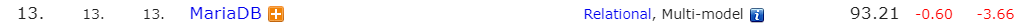
\includegraphics[width=\linewidth]{graphics/mariadbranking}
    \caption[MariaDB ranking]{MariaDB ranking~\autocite{DBEngines}}
    \label{fig:mariadbranking}
\end{figure}

\begin{figure}[H]
    \centering
    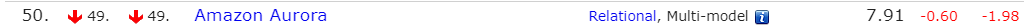
\includegraphics[width=\linewidth]{graphics/amazonauroraranking}
    \caption[Amazon Aurora ranking]{Amazon Aurora ranking~\autocite{DBEngines}}
    \label{fig:amazonauroraranking}
\end{figure}

Na zorgvuldige overweging en analyse werden nog drie andere databases geselecteerd om de shortlist van vijf databases aan te vullen. Deze databases zijn Couchbase, ClickHouse en MongoDB.
\begin{figure}[H]
    \centering
    \includegraphics[width=\linewidth]{"graphics/mongodb ranking"}
    \caption[MongoDB ranking]{MongoDB ranking~\autocite{DBEngines}}
    \label{fig:mongodb-ranking}
\end{figure}
\begin{figure}[H]
    \centering
    \includegraphics[width=\linewidth]{"graphics/couchbase ranking"}
    \caption[Couchbase ranking]{Couchbase ranking~\autocite{DBEngines}}
    \label{fig:couchbase-ranking}
\end{figure}
\begin{figure}[H]
    \centering
    \includegraphics[width=\linewidth]{"graphics/clickhouse ranking"}
    \caption[ClickHouse ranking]{ClickHouse ranking~\autocite{DBEngines}}
    \label{fig:clickhouse-ranking}
\end{figure}


Couchbase werd gekozen voor de key-features die aangeboden worden, speciaal voor retail en e-commerce. Deze key-features omvatten: ~\autocite{Couchbasea} 

\begin{itemize}
    \item Makkelijkere en betaalbaardere schaalbaarheid.
    \item Verbeterde prestaties dankzij een in-memory en gedistribueerde architectuur die sub-millisecond reactietijden levert.
    \item De hoge beschikbaarheid.
    \item Kostenbesparingen en versnelling van de time-to-market door flexibiliteit en operationele efficiëntie, waardoor bedrijven snel kunnen reageren op veranderende marktomstandigheden.
\end{itemize}

Met MariaDB en Amazon Aurora, twee relationele databases en de NoSQL database, Couchbase, ontbrak er nog een tweede NoSQL database. Hiervoor werd geopteerd voor MongoDB. MongoDB staat wereldwijd bekend als een van de meest prominente NoSQL-databases en staat ook gerangschikt op de vijfde plaats.

Als laatste database werd gekozen voor een kolom database, ClickHouse. ClickHouse werd gekozen vanwege zijn uitstekende prestaties, schaalbaarheid, betrouwbaarheid, flexibele architectuur, uitgebreide functionaliteiten en gebruiksvriendelijkheid. Het biedt razendsnelle verwerking van analytische queries, schaalt efficiënt mee met hardwarebronnen tot petabyte-schaal, ondersteunt betrouwbare replicatie over meerdere datacenters, en vereenvoudigt het schrijven van queries met een gebruiksvriendelijke SQL-dialect.~\autocite{ClickHousea}



\chapter{\IfLanguageName{dutch}{Vergelijkende studie}{comparing study}}%
\label{ch:vergelijkende-studie}

\section{\IfLanguageName{dutch}{Welke database is het meest geschikt voor een e-commercewinkel in de modebranche?}{Which database is best suited for an e-commerce shop in the fashion industry?}}%
\label{sec:}

Voor het vervolg van deze literatuurstudie zal er een vergelijking uitgevoerd worden tussen vijf verschillende databases en besloten worden welke database de beste oplossing is voor een e-commerce webshop in de mode industrie. De vergelijking zal vooral gebaseerd zijn op de prestaties en kosten van de desbetreffende databases. Uit de vergelijkingen zal ook blijken waarom gekozen werd voor deze specifieke databases. De desbetreffende databases die vergeleken  gaan worden zijn: MariaDB, ClickHouse, Couchbase, Amazon Aurora en MongoDB.

\section{\IfLanguageName{dutch}{MariaDB}{MariaDB}}%
\label{sec:MariaDB}

MariaDB is een relationele database die gebruikt kan worden voor verschillende doeleinden waaronder e-commerce. MariaDB is cloud-native  en biedt een hoge beschikbaarheid en schaalbaarheid.~\autocite{MariaDB} Bovendien is MariaDB open source wat betekent dat het gratis gebruikt kan worden. Cloud native is een softwarebenadering die toelaat om moderne applicaties te bouwen, te implementeren en te beheren in een cloud computing omgeving. Cloud computing is het leveren van computingservices - zoals servers, opslag, databases, netwerken, software, analyses en intelligentie - via het internet ("de cloud") om snellere innovatie, flexibele middelen en schaalvoordelen te bieden.~\autocite{Microsofta} Het gebruik van een cloud-native aanpak heeft enkele voordelen: de efficiëntie kan verhoogd worden, de kosten kunnen verlaagd worden doordat er geen nood is aan het investeren in dure fysieke infrastructuur en de beschikbaarheid van de applicaties kan verzekerd worden.~\autocite{Amazona} Bovenop de schaalbaarheid, beschikbaarheid en cloud-native aanpak biedt mariaDB ook nog ondersteuning voor meerdere workloads (transacties en analyses), alsook ondersteuning voor meerdere datatypes (relationeel en JSON).

\section{\IfLanguageName{dutch}{ClickHouse}{ClickHouse}}%
\label{sec:ClickHouse}

Clickhouse is een databasebeheersysteem, geen database. Dit zorgt ervoor dat tijdens runtime tabellen en databases gemaakt kunnen worden, gegevens geladen kunnen worden en queries uitgevoerd kunnen worden zonder de server opnieuw te moeten configureren en opnieuw op te starten.~\autocite{ClickHouse} ClickHouse is een kolom georiënteerd database management systeem, die de snelheid van analytische queries optimaliseert. De data in deze kolommen wordt gecomprimeerd hetgeen een belangrijke rol speelt in het verbeteren van de prestaties van de database. Daarnaast is clickhouse ook ontworpen om te kunnen werken op gewone harde schijven wat ervoor zorgt dat de kost per GB opslag enorm daalt.

\section{\IfLanguageName{dutch}{Couchbase}{Couchbase}}%
\label{sec:Couchbase}

Couchbase is een gedistribueerde NoSQL-clouddatabase onder andere ontwikkeld voor de retail en e-commerce industrie. Volgens ~\textcite{Couchbase} worden NoSQL databases steeds vaker gebruikt vanwege de groeiende focus op klantbeleving, wat een cruciaal competitief onderscheid vormt in de zakenwereld. In het middelpunt van deze revolutie liggen de grote gegevens van een bedrijf, samen met cloud-, mobiele-, sociale media- en IoT-toepassingen. Traditionele relationele databases zijn niet meer in staat om te voldoen aan de groeiende eisen van moderne web-, mobiele- en IoT-toepassingen, zoals bijvoorbeeld het ondersteunen van grote aantallen gebruikers, hoge responsiviteit, continue beschikbaarheid en het verwerken van semi- en ongestructureerde data. Dit heeft geleid tot een groeiende adoptie van NoSQL-databases door grote bedrijven zoals Tesco, Marriott, Gannett en GE. De opkomst van vijf trends in de digitale economie - zoals meer online klanten en de groei van big data - heeft geleid tot nieuwe technische uitdagingen die NoSQL-databases kunnen oplossen. Ondertussen blijven traditionele relationele databases achter omdat ze niet voldoen aan de vereisten van een snel veranderende digitale economie en niet geschikt zijn voor agile ontwikkeling. Door de netwerkgerichte architectuur van couchbase is ook de prijs voor het schalen van een dergelijke database goedkoper en eenvoudiger. Daarnaast biedt couchbase ook hoge prestaties en efficiëntie door hun in memory en gedistribueerde architectuur.~\autocite{Couchbasea}

\newpage

\section{\IfLanguageName{dutch}{Amazon Aurora}{Amazon Aurora}}%
\label{sec:Amazon Aurora}

Amazon Aurora is een relationele databaseservice die de snelheid en beschikbaarheid van high-end commerciële databases combineert met eenvoud en kosteneffectiviteit.~\autocite{Amazonb} Volgens~\textcite{Amazonb} zou er een toename in doorvoer zijn van maximaal 5x ten opzichte van de standaard MySQL. Dankzij de serverless configuratie voor Amazon Aurora is het ook mogelijk om de database automatisch te schalen op basis van de vereisten van het bedrijf. 

\section{\IfLanguageName{dutch}{MongoDB Atlas}{MongoDB Atlas}}%
\label{sec:MongoDB Atlas}

Zoals eerder besproken bij couchbase wordt het gebruik van een NoSQL database voor een e-commerce website steeds populairder. Vandaar ook de keuze voor MongoDB Atlas. MongoDB Atlas is een multi-cloud databaseservice aangeboden door mongoDB. Atlas zorgt voor een vereenvoudigde implementatie en beheer van de database en biedt tegelijkertijd de veelzijdigheid die nodig is om een veerkrachtige en performante applicatie te bouwen op een cloudprovider.~\autocite{MongoDBa} MongoDB Atlas biedt toegang tot alle core features die MongoDB aanbiedt. Hieronder valt onder meer de hoge prestaties, de schaalbaarheid, de hoge beschikbaarheid en meer. ~\autocite{MongoDBb}

\section{\IfLanguageName{dutch}{Conclusie}{Conclusion}}%
\label{sec:Conclusie}

Op basis van de geraadpleegde literatuur kan besloten worden dat voor het bouwen van een moderne e-commerce website, in dit geval in de mode-industrie best gebruik gemaakt wordt van een NoSQL database. Dit mede om te kunnen voldoen aan de voortdurende groei aan vraag van de klanten. Dit betekent dat zowel MariaDB, Clickhouse en Amazon Aurora uitgesloten kunnen worden. Zowel MongoDb atlas als Couchbase zijn een uitstekende oplossing. Couchbase geniet hierbij de voorkeur aangezien het goede prestaties en gemakkelijke schaling aanbiedt. Couchbase is echter niet goedkoop. De goedkoopste service die momenteel aangeboden wordt is \$0,28/uur (€0,26/uur), wat ongeveer overeen komt met \$201,6/maand (€189,00/maand). MongoDB Atlas daarentegen biedt al services aan vanaf \$57/maand (€53,44/maand). Dit is ongeveer 1/4 de van de prijs van Couchbase. Als startup is het dus mogelijks interessanter om te beginnen met een MongoDB Atlas database. Indien geld een minder belangrijke rol speelt, wordt aangeraden om een Couchbase database te gebruiken.


\begin{table}[H]
    \centering
    \begin{tabular}{l S[table-format=1.2] S[table-format=1.2] S[table-format=3.2] S[table-format=3.2]}
        \toprule
        \textbf{Service} & \textbf{Prijs/u (\$)} & \textbf{Prijs/u (€)} & \textbf{Prijs/mnd (\$)} & \textbf{Prijs/mnd (€)} \\
        \midrule
        Couchbase & 0.28 & 0.26 & 201.60 & 189.00 \\
        MongoDB Atlas & \multicolumn{2}{c}{N.v.t.} & 57.00 & 53.44 \\
        \bottomrule
    \end{tabular}
    \caption{Vergelijking van kosten tussen Couchbase en MongoDB Atlas}
    \label{tab:prices}
\end{table}

De prijzen voor Amazon Aurora en ClickHouse zijn gebaseerd op het verbruik en de configuraties die gemaakt worden (totaal geheugen, opslag, enzovoort).


\chapter{\IfLanguageName{dutch}{Testopstelling/PoC}{Test/PoC}}%
\label{ch:onderzoek}

\section{\IfLanguageName{dutch}{Opzetten testopstelling}{Creating test environment}}%
\label{sec:testopstelling}

Voor het opzetten van de testopstelling is een gratis trial aangegaan voor elk van de gekozen vijf databases. Deze omvatten: MariaDB, ClickHouse, Couchbase, Amazon Aurora en MongoDB Atlas.

Door het bedrijf Aware werd een statistiek ter beschikking gesteld met betrekking tot de uitgevoerde queries. Dit wordt weergegeven in figuur~\ref{fig:statistics}.

\begin{figure}[H]
    \centering
    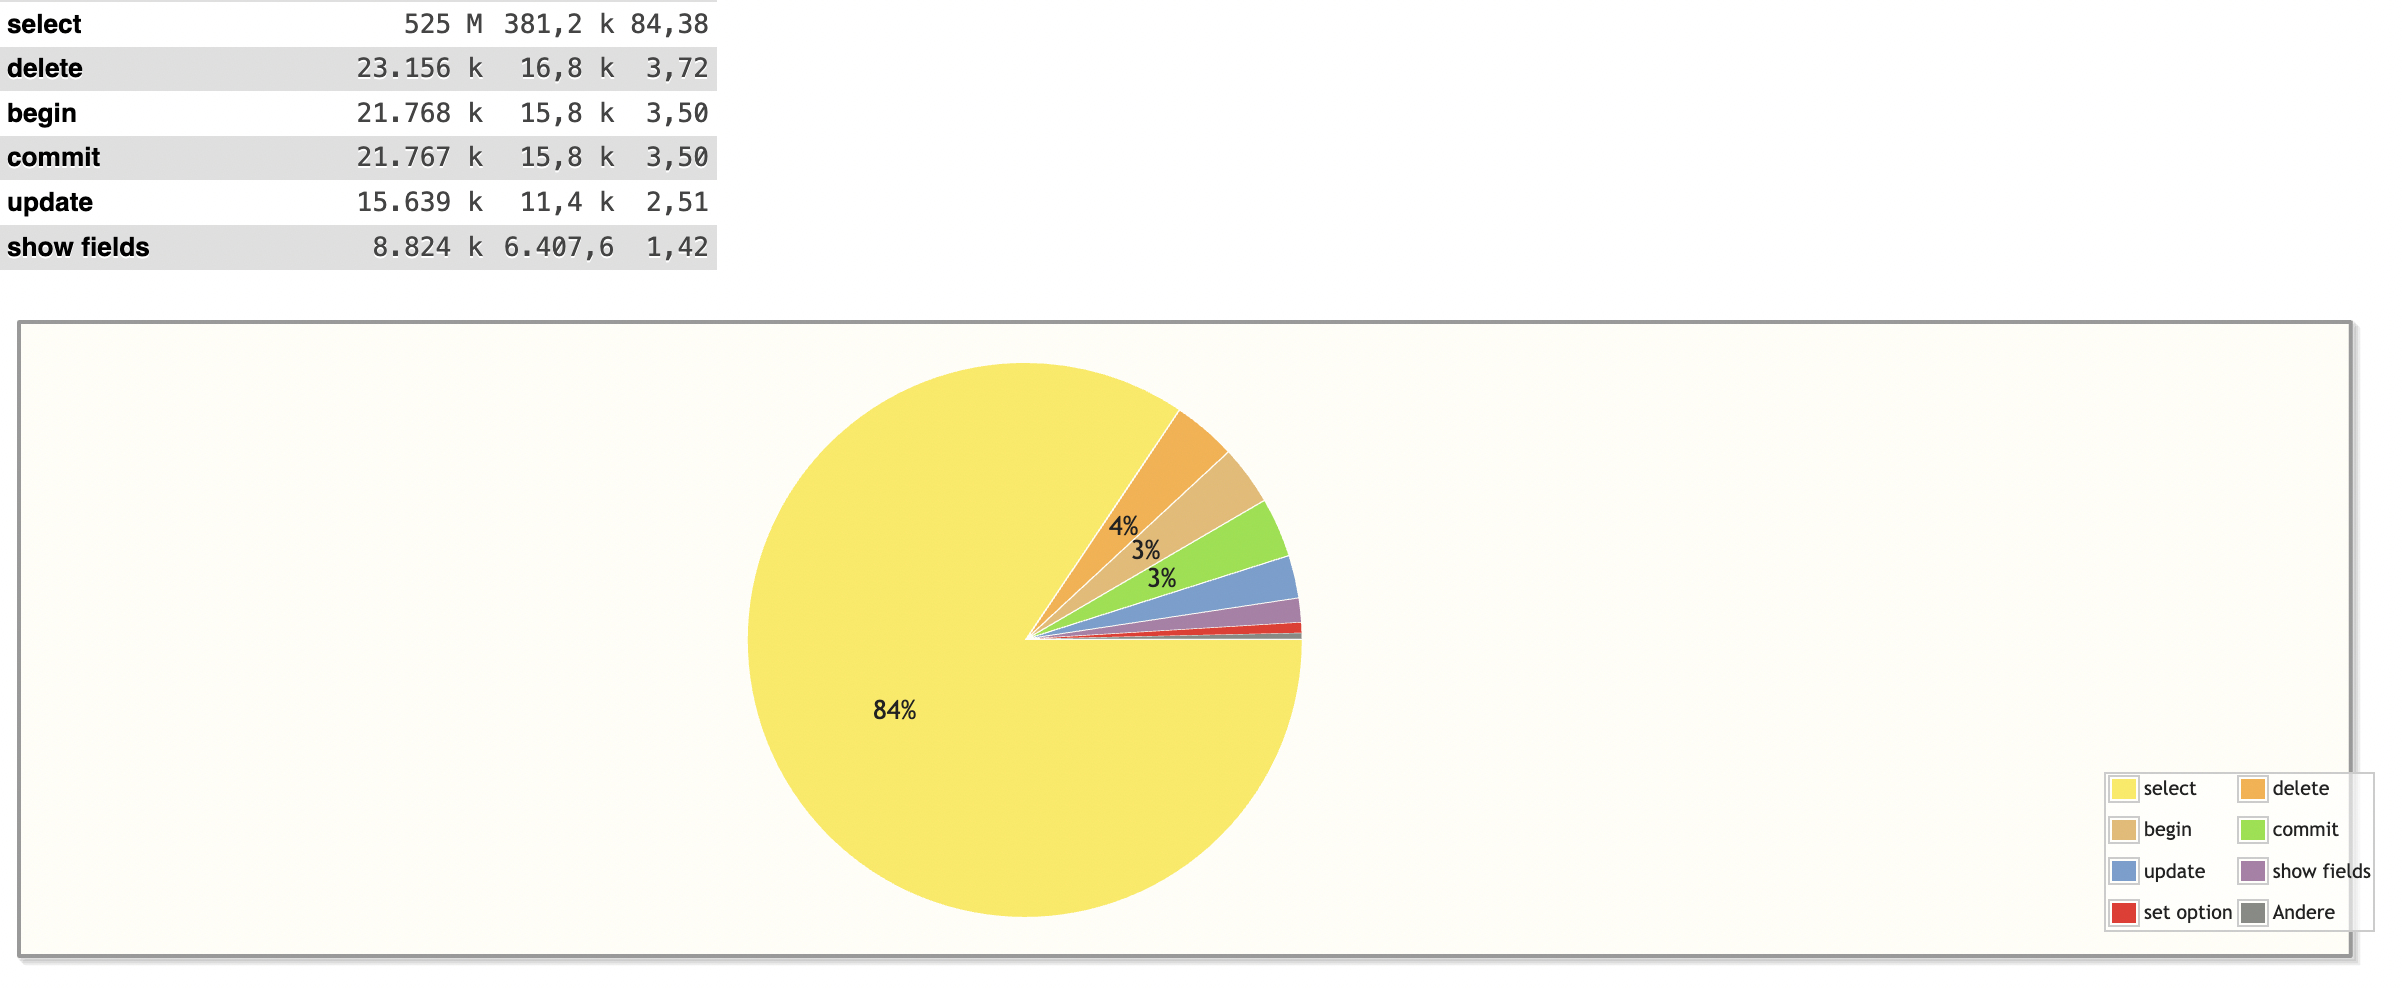
\includegraphics[width=\linewidth]{graphics/statistics}
    \caption[Query statistieken Aware]{Query statistieken Aware | mei 2023 - maart 2024}
    \label{fig:statistics}
\end{figure}

Op basis van verkregen statistieken van het bedrijf Aware, kan afgeleid worden dat het merendeel van de uitgevoerde queries, select queries zijn. Tijdens het testen zal hier dan ook de nadruk op gelegd worden. 

Voor het testen van de database prestaties is het belangrijk te definiëren welke statistieken gemeten en gemonitord moeten worden. Tijdens de testen zal er vooral gefocust worden op de response time, de tijd die de database erover doet om een query of een transactie uit te voeren en de gevonden resultaten terug te geven aan de gebruiker. 

Zoals eerder besproken in de stand van zaken wordt er vanuit gegaan dat een e-commerce webshop in de mode-industrie volgende gegevens opslaat: 

\begin{itemize}
    \item Klanten
    \item Producten
    \item Categorieën
    \item Bestellingen
    \item Bestelitems
    \item Betaalmethoden
    \item Verzendmethoden
    \item Voorraad
    \item Logs
\end{itemize}
Om de database op te vullen met deze gegevens werd er random data gegenereerd voor deze gegevens.

\newpage

\section{\IfLanguageName{dutch}{MariaDB}{MariaDB}}%
\label{sec:test-mariadb}

\subsection{\IfLanguageName{dutch}{Opzetten van de database}{Creating the database}}%
\label{subsec:creating-mariadb}

Nadat de MariaDB-client is geïnstalleerd, werd een terminal geopend waarin enkele commando's werden uitgevoerd om een nieuwe database aan te maken. In Figuur~\ref{fig:mariadbconnection} wordt een dergelijke terminal geïllustreerd waarin al een verbinding met de MariaDB-client is gemaakt.

\begin{figure}[H]
    \centering
    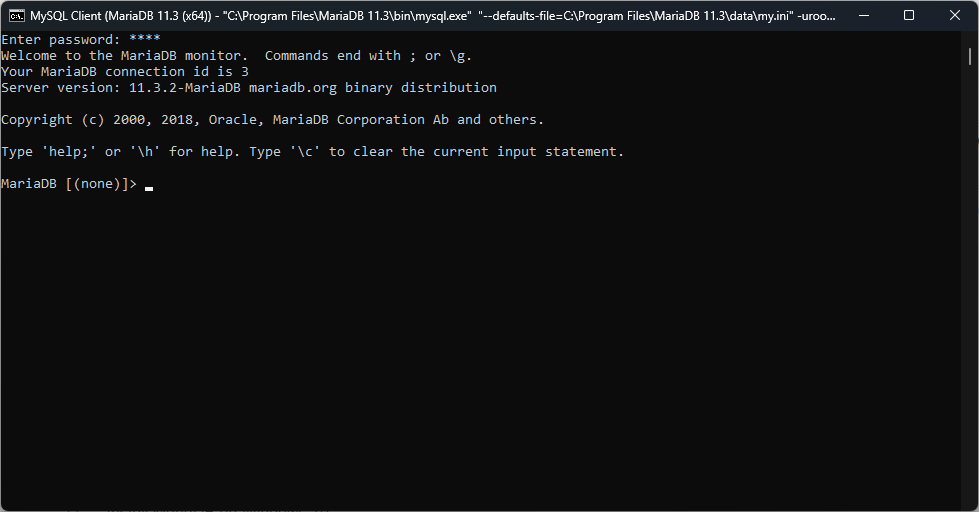
\includegraphics[width=\linewidth]{graphics/mariadbconnection}
    \caption[Terminal met een actieve verbinding met de MariaDB-client.]{Terminal met een actieve verbinding met de MariaDB-client.}
    \label{fig:mariadbconnection}
\end{figure}

Er kan een database in de MariaDB-client worden aangemaakt door volgend commando uit te voeren:

\begin{lstlisting}[language=SQL, caption={SQL-query voor het aanmaken van de database.}]
    CREATE DATABASE mariadbtest;
\end{lstlisting}

Voor het opstellen van het schema van de database werd vooraf een eenvoudig Entity-Relationship Diagram (ERD) opgesteld, zoals te zien is in Figuur~\ref{fig:erd-e-commerce}. Dit ERD diende als basis voor het opstellen van de database.

\begin{figure}[H]
    \centering
    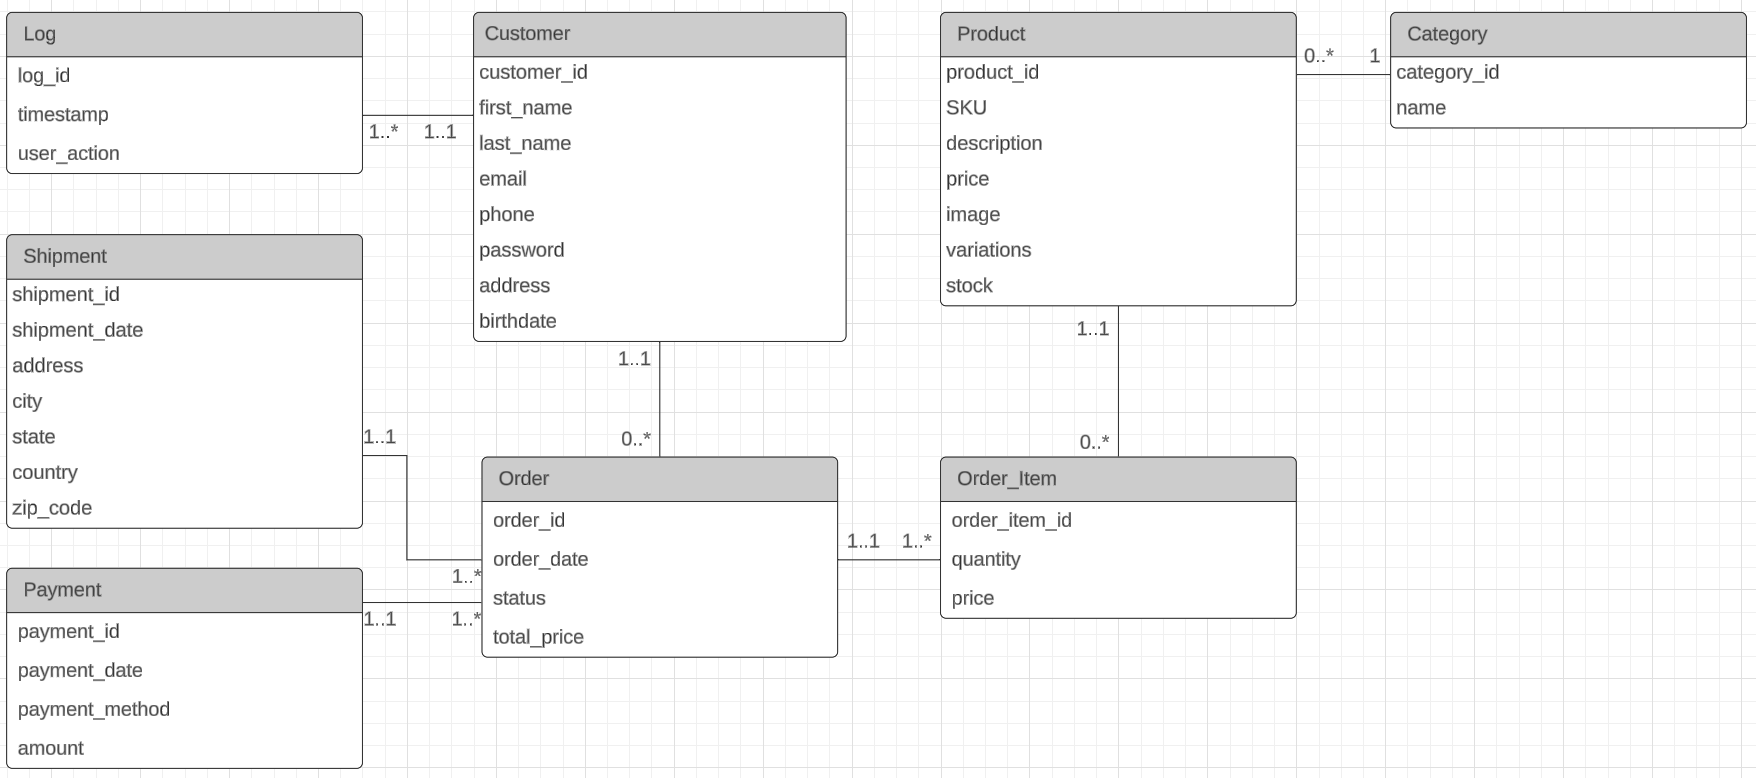
\includegraphics[width=\linewidth]{graphics/erd-e-commerce}
    \caption[Entity-Relationship Diagram (ERD) voor het e-commerce project.]{Entity-Relationship Diagram (ERD) voor het e-commerce project.}
    \label{fig:erd-e-commerce}
\end{figure}

Om de tabellen in de database te maken, werden volgende commando's uitgevoerd:

\begin{lstlisting}[language=SQL, caption={SQL-queries voor het aanmaken van de categorie en product tabel in de database.}]
    CREATE TABLE Category (
    category_id INTEGER AUTO_INCREMENT,
    name VARCHAR(50) NOT NULL,
    PRIMARY KEY (category_id)
    );
    
    CREATE TABLE Product (
    product_id INTEGER AUTO_INCREMENT,
    category_id INTEGER,
    SKU VARCHAR(50),
    description VARCHAR(255),
    price DECIMAL(10, 2),
    stock INTEGER,
    image VARCHAR(255),
    variations JSON,
    PRIMARY KEY (product_id),
    FOREIGN KEY (category_id) REFERENCES Category(category_id)
    );
\end{lstlisting}

Na het uitvoeren van alle commando's werd een schema zoals weergegeven in Figuur~\ref{fig:mariadb} verkregen.

\begin{figure}[H]
    \centering
    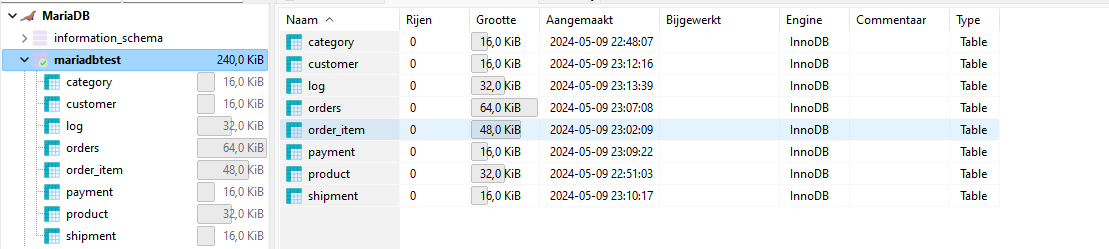
\includegraphics[width=\linewidth]{graphics/mariadb}
    \caption[Schema van de database na het aanmaken van de tabellen.]{Schema van de database na het aanmaken van de tabellen.}
    \label{fig:mariadb}
\end{figure}

Voordat er testen kunnen worden uitgevoerd, moet er data in de database worden ingevoerd. Dit kan met behulp van het volgende commando:

\begin{lstlisting}[language=SQL, caption={SQL-query voor het invoegen van nieuwe categorieën in de database.}]
    INSERT INTO Category (name) VALUES
    ('Kleding'),
    ('Schoenen'),
    ('Accessoires'),
    ('Handtassen'),
    ('Sieraden'),
    ('Horloges'),
    ('Sportkleding'),
    ('Zwemkleding'),
    ('Ondergoed'),
    ('Nachtkleding'),
    ('Werkkleding'),
    ('Feestkleding'),
    ('Casual kleding'),
    ('Vintage kleding'),
    ('Duurzame kleding'),
    ('Plus-size kleding'),
    ('Kinderkleding'),
    ('Babykleding'),
    ('Herenkleding'),
    ('Dameskleding');
\end{lstlisting}

Nadat er voldoende data ($\pm$ 3.8 miljoen rijen) is geïmporteerd, kunnen er testen worden uitgevoerd. Als voorbeeld wordt een SELECT-query uitgevoerd om alle producten te tonen die zijn geassocieerd met de categorie "Schoenen", gevolgd door een query om een schoen bij te werken, toe te voegen en te verwijderen.

\begin{lstlisting}[language=SQL, caption={SQL-queries voor het beheren van producten in de database.}]
    -- Query 1: Ophalen van alle producten voor een bepaalde categrorie.
    SELECT p.product_id, p.SKU, p.description, p.price, p.stock,
     p.image, c.name AS category_name
    FROM Product p
    JOIN Category c ON p.category_id = c.category_id
    WHERE c.name = 'Schoenen';
    
    -- Query 2: Update van een product
    UPDATE Product
    SET description = 'Nieuwe beschrijving', price = 49.99, stock = 100
    WHERE product_id = 1;
    
    -- Query 3: Toevoegen van een nieuw product
    INSERT INTO Product 
    (category_id, SKU, description, price, stock, image, variations)
    VALUES 
    (1, 'SKU123', 'Nieuw product', 39.99, 50, 'product_image.jpg', 
    '{"size": "L", "color": "blue"}');
    
    -- Query 4: Verwijderen van een product
    DELETE FROM Product
    WHERE product_id = 2;
\end{lstlisting}
\subsection{\IfLanguageName{dutch}{Resultaten}{Results}}%
\label{subsec:results}

Na het uitvoeren van de verschillende queries werden de volgende resultaten verkregen:

\begin{table}[htbp]
    \centering
    \caption{Gemiddelde tijden voor SELECT SQL-operaties}
    \begin{tabularx}{\textwidth}{*{8}{>{\centering\arraybackslash}X}c}
        \toprule
        \multicolumn{8}{c}{Tijd (s)} & Gemiddelde \\
        \midrule
        4,891 & 5,141 & 4,593 & 4,422 & 4,484 & 4,547 & 4,047 & 4,312 & 4,479 \\
        4,469 & 4,422 & 4,390 & 4,454 & 4,406 & 4,360 & 4,579 & & \\
        \bottomrule
    \end{tabularx}
\end{table}

\begin{figure}[H]
    \centering
    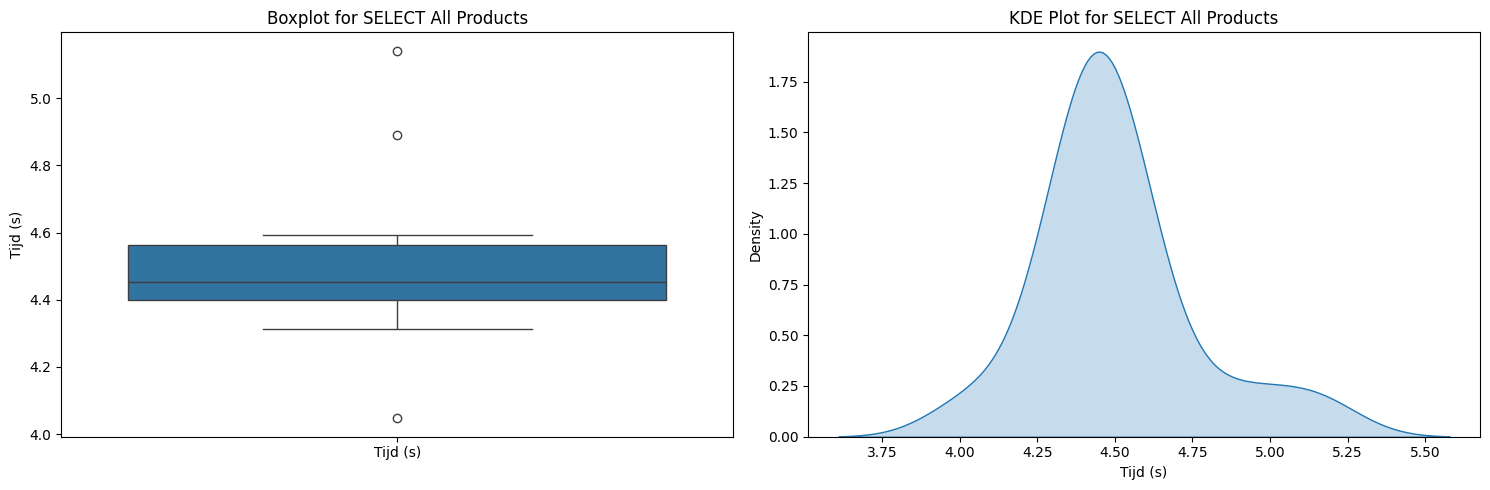
\includegraphics[width=\linewidth]{graphics/plots-slect-all-mariadb}
    \caption[Box- en KDE-plot select all MariaDB]{Box- en KDE-plot voor het ophalen van alle producten in MariaDB}
    \label{fig:plots-slect-all-mariadb}
\end{figure}

\begin{table}[htbp]
    \centering
    \caption{Gemiddelde tijden voor SELECT + JOIN + WHERE SQL-operaties}
    \begin{tabularx}{\textwidth}{*{8}{>{\centering\arraybackslash}X}c}
        \toprule
        \multicolumn{8}{c}{Tijd (s)} & Gemiddelde \\
        \midrule
        4,875 & 4,875 & 4,844 & 4,859 & 4,859 & 4,844 & 4,891 & 4,719 & 4,836 \\
        4,922 & 4,781 & 4,875 & 4,828 & 4,734 & 4,859 & 4,828 & & \\
        \bottomrule
    \end{tabularx}
\end{table}
\begin{figure}[H]
    \centering
    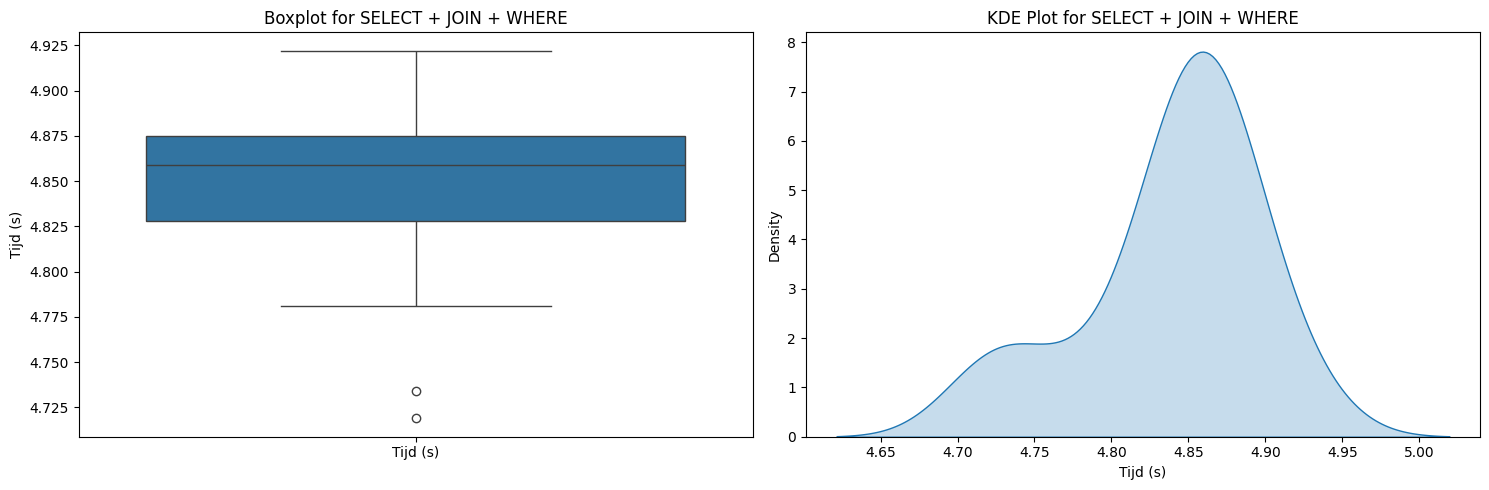
\includegraphics[width=\linewidth]{graphics/plots-slect-join-mariadb}
    \caption[Box- en KDE-plot select where MariaDB]{Box- en KDE-plot voor het selecteren van alle producten die vasthagen aan een bepaalde categorie in MariaDB}
    \label{fig:plots-slect-join-mariadb}
\end{figure}

\begin{table}[htbp]
    \centering
    \caption{Gemiddelde tijden voor BULK INSERT SQL-operaties}
    \begin{tabularx}{\textwidth}{*{8}{>{\centering\arraybackslash}X}c}
        \toprule
        \multicolumn{8}{c}{Tijd (s)} & Gemiddelde \\
        \midrule
        0,015 & 0,000 & 0,000 & 0,000 & 0,016 & 0,016 & 0,016 & 0,000 & 0,006 \\
        0,016 & 0,000 & 0,000 & 0,016 & 0,000 & 0,000 & 0,016 & & \\
        \bottomrule
    \end{tabularx}
\end{table}
\begin{figure}[H]
    \centering
    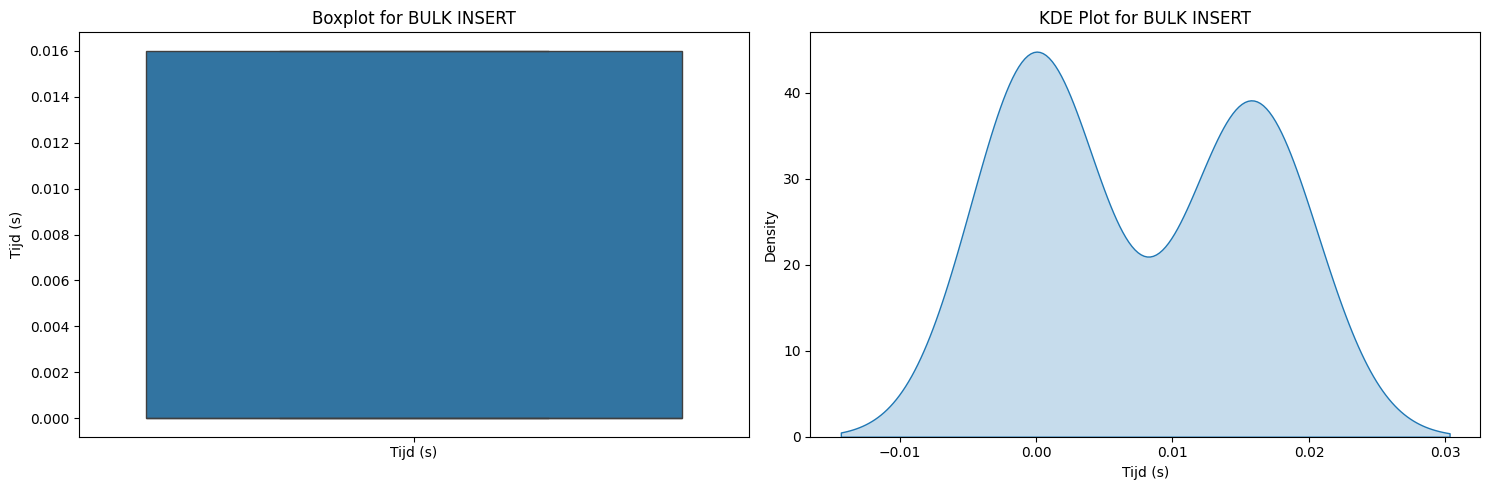
\includegraphics[width=\linewidth]{graphics/plots-insert-mariadb}
    \caption[Box- en KDE-plot insert MariaDB]{Box- en KDE-plot voor het toevoegen van een product in MariaDB}
    \label{fig:plots-insert-mariadb}
\end{figure}

\begin{table}[htbp]
    \centering
    \caption{Gemiddelde tijden voor UPDATE + WHERE SQL-operaties}
    \begin{tabularx}{\textwidth}{*{8}{>{\centering\arraybackslash}X}c}
        \toprule
        \multicolumn{8}{c}{Tijd (s)} & Gemiddelde \\
        \midrule
        11,562 & 11,625 & 12,281 & 12,109 & 12,375 & 12,109 & 12,359 & 11,406 & 11,865 \\
        12,141 & 11,250 & 11,765 & 11,875 & 12,141 & 11,734 & 11,473 & & \\
        \bottomrule
    \end{tabularx}
\end{table}
\begin{figure}[H]
    \centering
    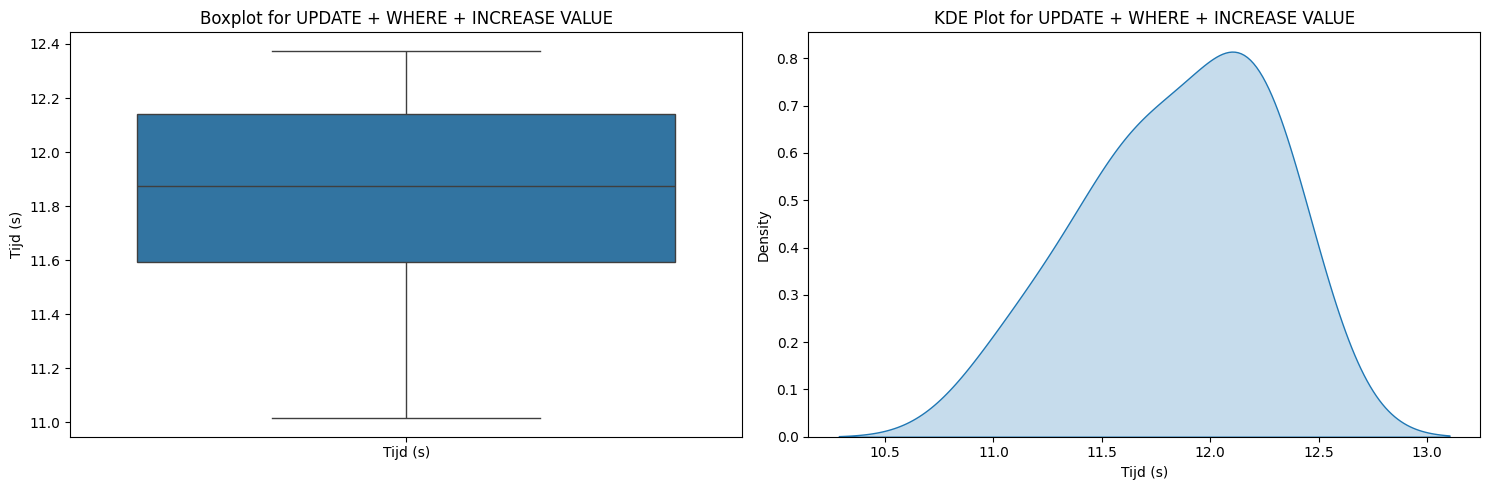
\includegraphics[width=\linewidth]{graphics/plots-update-mariadb}
    \caption[Box- en KDE-plot update where MariaDB]{Box- en KDE-plot voor het verhogen van een waarde van een product in MariaDB}
    \label{fig:plots-update-mariadb}
\end{figure}

\begin{table}[htbp]
    \centering
    \caption{Gemiddelde tijden voor DELETE SQL-operaties}
    \begin{tabularx}{\textwidth}{*{8}{>{\centering\arraybackslash}X}c}
        \toprule
        \multicolumn{8}{c}{Tijd (s)} & Gemiddelde \\
        \midrule
        0,015 & 0,000 & 0,000 & 0,000 & 0,000 & 0,000 & 0,000 & 0,015 & 0,004 \\
        0,000 & 0,000 & 0,000 & 0,000 & 0,015 & 0,015 & 0,000 & & \\
        \bottomrule
    \end{tabularx}
\end{table}

\begin{figure}[H]
    \centering
    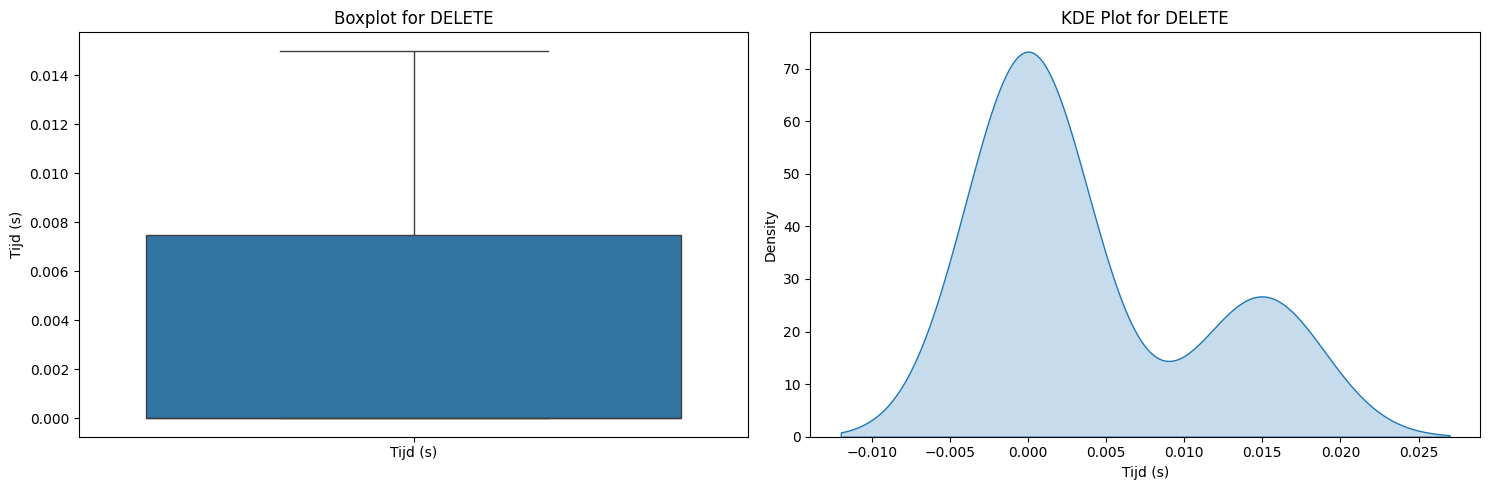
\includegraphics[width=\linewidth]{graphics/plots-delete-mariadb}
    \caption[Box- en KDE-plot delete MariaDB]{Box- en KDE-plot voor het verwijderen van een product in MariaDB}
    \label{fig:plots-delete-mariadb}
\end{figure}


\newpage




\section{\IfLanguageName{dutch}{MongoDB}{MongoDB}}%
\label{sec:test-mongodb}

\subsection{\IfLanguageName{dutch}{Opzetten database}{Creating database}}%
\label{subsec:creating-mongodb}

Voor het opzetten van de MongoDB-database is de bestaande data uit de MariaDB-database geëxporteerd naar een CSV-bestand. Enkel een deel van deze data kon geexporteerd worden alvorens een error optrad. ($\pm$ 1.9 miljoen rijen) Dit bestand is vervolgens geïmporteerd in het vooraf geïnstalleerde MongoDB Compass-programma. Vanwege de beperkte opslagcapaciteit van de gratis ter beschikking gestelde database kon slechts een deel van de gegevens worden geïmporteerd. ($\pm$ 1.5 miljoen rijen) Dit kan leiden tot afwijkingen in de gemeten data ten opzichte van onder andere de resultaten van MariaDB. Ondanks deze beperking kunnen de verkregen resultaten nog steeds nuttig zijn.

Figuur \ref{fig:mongodbsetup} toont de setup van de MongoDB-database, waarin de opslaggrootte van 52.6 MB, de logische gegevensgrootte, en het aantal documenten te zien zijn.

\begin{figure}[H]
    \centering
    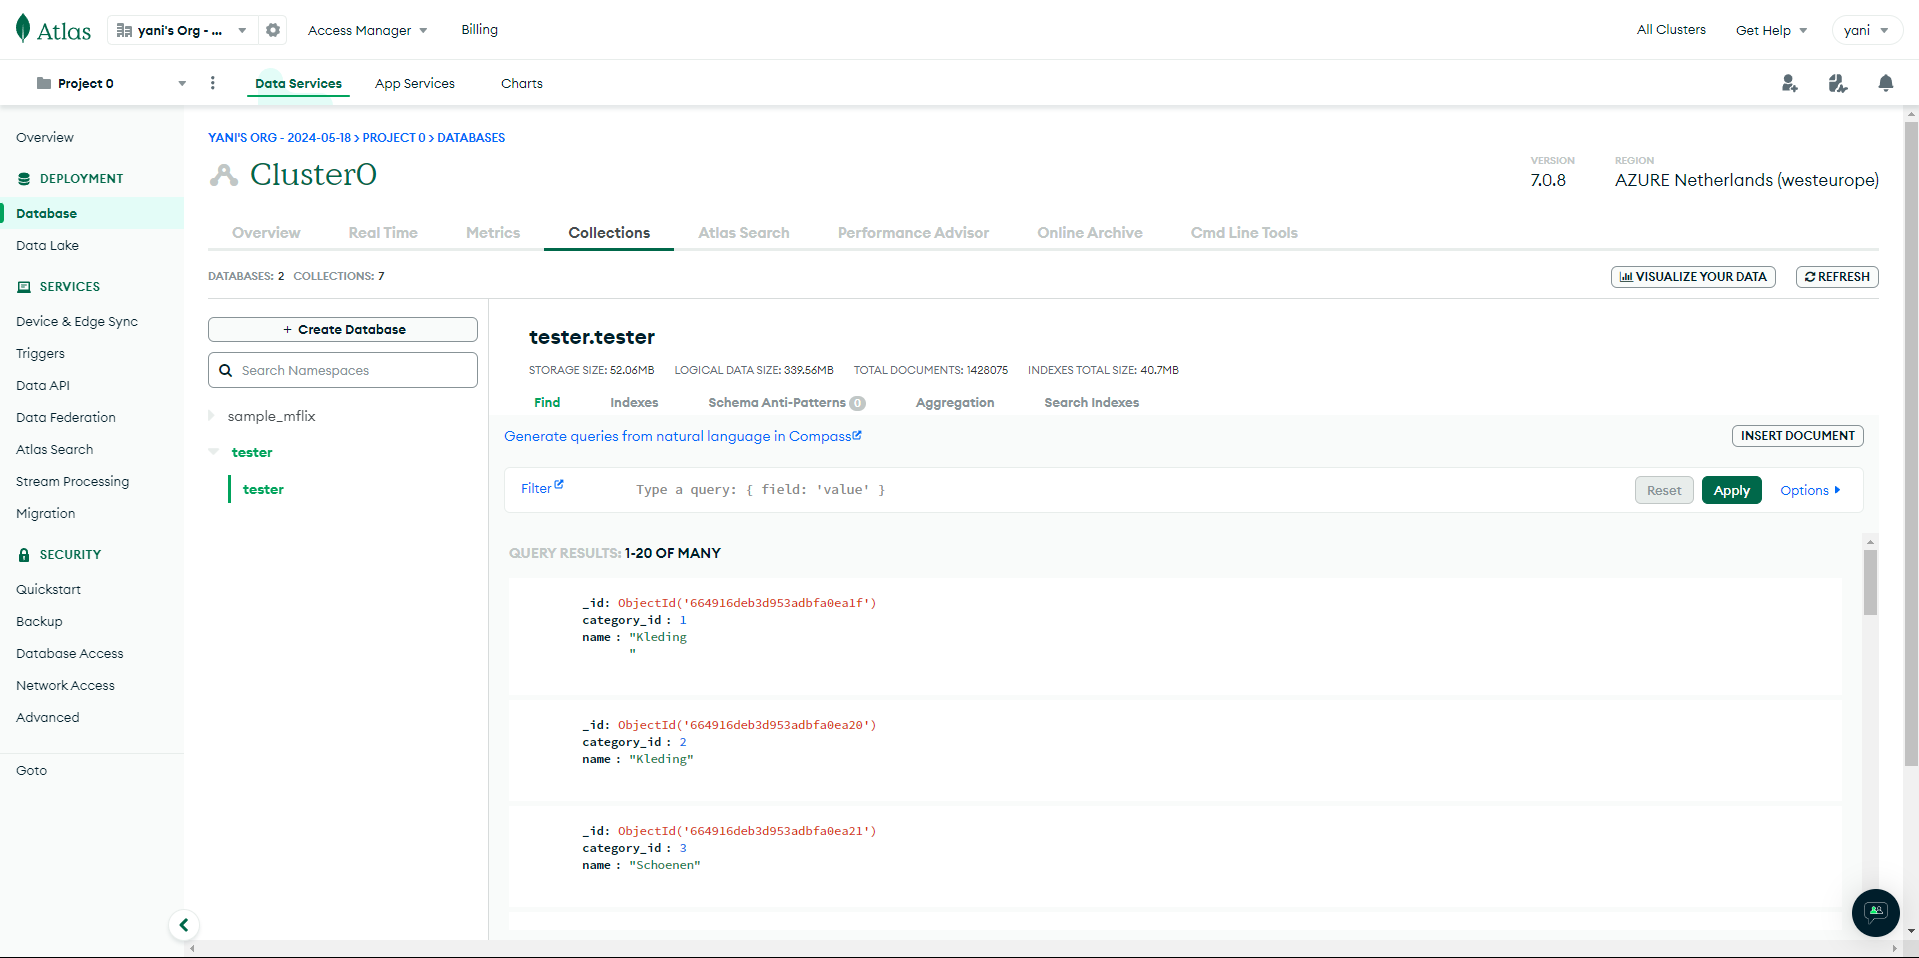
\includegraphics[width=\linewidth]{graphics/mongodbsetup}
    \caption[MongoDB setup]{MongoDB setup}
    \label{fig:mongodbsetup}
\end{figure}

\newpage

Voor het bekomen van de resultaten werden enkele queries opgesteld. Hieronder worden enkele voorbeelden weergegeven:
\begin{lstlisting}[language=NOSQL, caption={MongoDB-queries voor het beheren van producten in de database.}]
    -- Query 1: Ophalen van alle producten voor een bepaalde categorie.
    {'category_id': 3}
    
    -- Query 2: Update van een product
    db.products.updateOne(
    { product_id: 1 },
    {
        $set: {
            description: 'Nieuwe beschrijving',
            price: 49.99,
            stock: 100
        }
    }
    );
    
    -- Query 3: Toevoegen van een nieuw product
    db.products.insertOne({
        category_id: 1,
        SKU: 'SKU123',
        description: 'Nieuw product',
        price: 39.99,
        stock: 50,
        image: 'product_image.jpg',
        variations: {
            size: 'L',
            color: 'blue'
        }
    });
    
    -- Query 4: Verwijderen van een product
    db.products.deleteOne({ product_id: 2 });
\end{lstlisting}

\newpage

\subsection{\IfLanguageName{dutch}{Resultaten}{Results}}%
\label{subsec:results2}

Na het uitvoeren van de verschillende queries werden voor MongoDB volgende resultaten verkregen:

\begin{table}[htbp]
    \centering
    \caption{Gemiddelde tijden voor SELECT all - {}}
    \begin{tabularx}{\textwidth}{*{8}{>{\centering\arraybackslash}X}c}
        \toprule
        \multicolumn{8}{c}{Tijd (s)} & Gemiddelde \\
        \midrule
        0,977 & 0,945 & 0,929 & 0,921 & 0,997 & 0,940 & 0,926 & 1,050 & 0,964 \\
        0,950 & 0,910 & 0,835 & 0,864 & 1,036 & 0,825 & 0,865 & & \\
        \bottomrule
    \end{tabularx}
\end{table}

\begin{figure}[H]
    \centering
    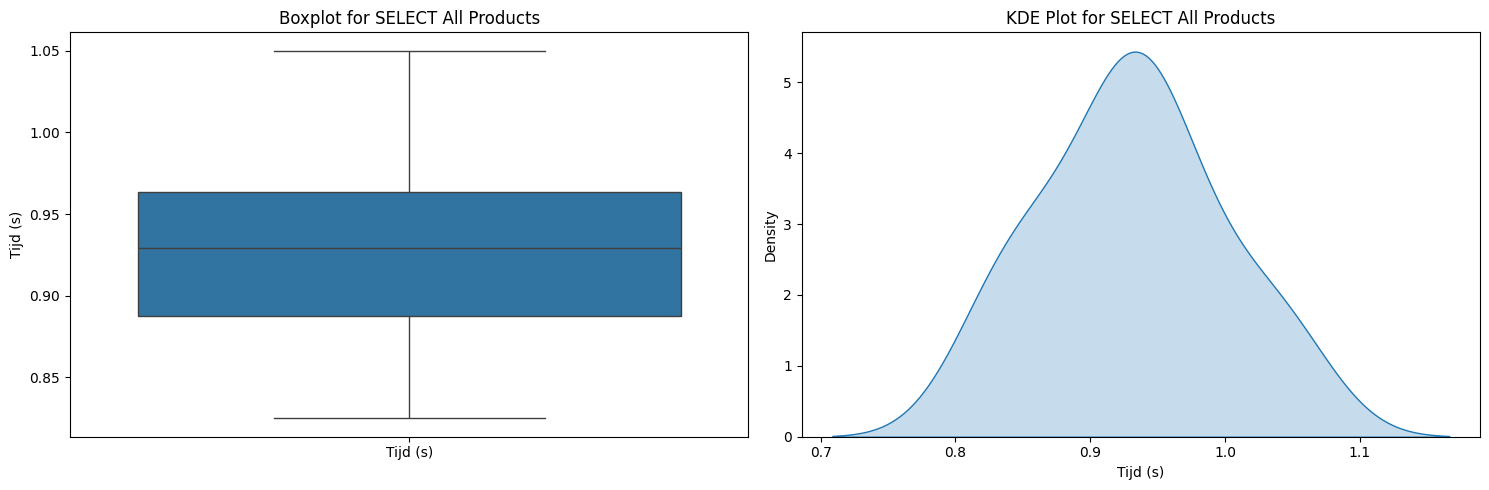
\includegraphics[width=\linewidth]{graphics/mongodb-select-all}
    \caption[Box- en KDE-plot select all MongoDB]{Box- en KDE-plot voor het selecteren van alle producten uit MongoDB.}
    \label{fig:mongodb-select-all}
\end{figure}


\begin{table}[htbp]
    \centering
    \caption{Gemiddelde tijden voor SELECT where - { "category_id": 3 }}
    \begin{tabularx}{\textwidth}{*{8}{>{\centering\arraybackslash}X}c}
        \toprule
        \multicolumn{8}{c}{Tijd (s)} & Gemiddelde \\
        \midrule
        1,399 & 1,509 & 1,385 & 1,288 & 1,289 & 1,386 & 1,291 & 1,270 & 1,353 \\
        1,272 & 1,265 & 1,362 & 1,454 & 1,271 & 1,284 & 1,253  & & \\
        \bottomrule
    \end{tabularx}
\end{table}

\begin{figure}[H]
    \centering
    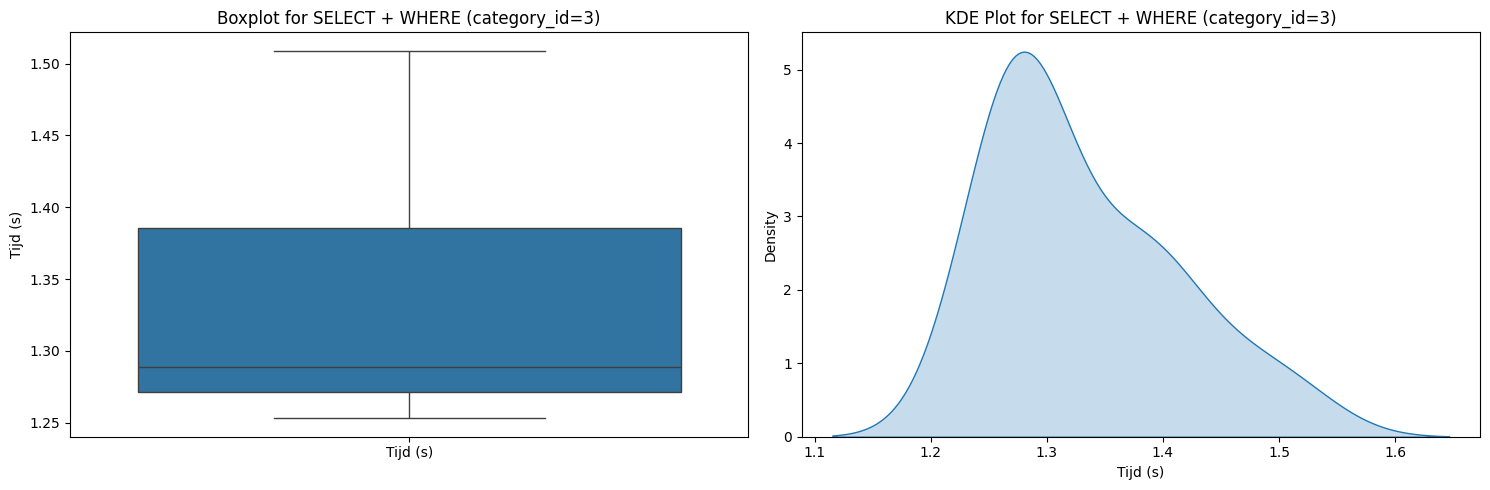
\includegraphics[width=\linewidth]{graphics/mongodb-select-category}
    \caption[Box- en KDE-plot select all where MongoDB]{Box- en KDE-plot voor het selecteren van alle producten waar de categorie id gelijk is aan 3 in MongoDB}
    \label{fig:mongodb-select-category}
\end{figure}

Voor MongoDB zijn er geen statistieken beschikbaar voor insert-, update- en delete-queries. Naast de maximale grootte van de database in de gratis versie, is er ook een beperking op het uitvoeren van bepaalde commando's. Een van deze commando's is het aanpassen van het profileringsniveau. Dit verhindert dat de uitvoeringssnelheid en andere statistieken van alle uitgevoerde queries beschikbaar worden gemaakt. Omdat gebruik werd gemaakt van de gratis versie, konden de querystatistieken alleen worden bekeken voor select-queries. In figuur \ref{fig:mongodberror} zijn het betreffende commando en de foutcode te vinden.

\begin{figure}[H]
    \centering
    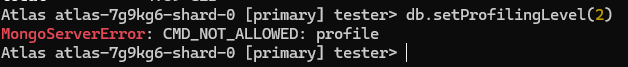
\includegraphics[width=\linewidth]{graphics/mongodberror}
    \caption[MongoDB foutcode]{MongoDB foutcode uitvoeren setProfilingLevel}
    \label{fig:mongodberror}
\end{figure}



\newpage



\section{\IfLanguageName{dutch}{Couchbase}{couchbase}}%
\label{sec:test-couchbase}

\subsection{\IfLanguageName{dutch}{Opzetten database}{Creating database}}%
\label{subsec:creating-couchbase}

Net zoals bij het opzetten van de MongoDB-database, werd voor het opzetten van de Couchbase-database een CSV-bestand gebruikt. Couchbase had echter een limiet op de grootte van deze bestanden, namelijk 40 MB. Dit betekende dat het slechts mogelijk was om maximaal 40 MB aan data te importeren.

\begin{figure}[H]
    \centering
    \includegraphics[width=\linewidth]{"graphics/Couchbase query"}
    \caption[Voorbeeld couchbase query]{Voorbeeld Couchbase query}
    \label{fig:couchbase-query}
\end{figure}

Figuur \ref{fig:couchbase-query} toont een screenshot van de Couchbase-datatools waarin de testen werden uitgevoerd. In de screenshot is ook een voorbeeld van een query te vinden, inclusief de uitvoeringstijd en hoe deze tijd wordt bepaald.

Hieronder volgen enkele gebruikte queries:

 \begin{lstlisting}[language=SQL, caption={Couchbase-queries voor het beheren van producten in de database.}]
     -- Query 1: Select all products
     SELECT * FROM fashion.`_default`.products;
     
     -- Query 2: Toevoegen van een product
     INSERT INTO `products` (KEY, VALUE)
     VALUES (UUID(), 
     {"c1": 2, "c2": "Home Appliances", "c3": "Refrigerators", 
         "c4": "Energy Efficient", "c5": 50,
          "c6": "Active", "c7": "2023-04-02", "c8": 300});
     
     -- Query 3: Updaten van een product
     UPDATE `products` SET c5 = c5 + 1 WHERE META().id = "3";
     
     -- Query 4: Verwijderen van een product
     DELETE FROM `products` WHERE META().id = "3";
 \end{lstlisting}


\subsection{\IfLanguageName{dutch}{Resultaten}{Results}}%
\label{subsec:results3}

Na het uitvoeren van de verschillende queries werden voor Couchbase volgende resultaten verkregen.

\begin{table}[htbp]
    \centering
    \caption{Gemiddelde tijden voor SELECT * FROM fashion.\_default.categories}
    \begin{tabularx}{\textwidth}{*{8}{>{\centering\arraybackslash}X}c}
        \toprule
        \multicolumn{8}{c}{Tijd (s)} & Gemiddelde \\
        \midrule
        7.9 & 12.8 & 18.9 & 9.4 & 9.8 & 10.7 & 15.4 & 8.7 & 11.8 \\
        13.5 & 8.4 & 10.1 & 14.7 & 23.1 & 8.9 & 10.2 & & \\
        \bottomrule
    \end{tabularx}
\end{table}

\begin{figure}[H]
    \centering
    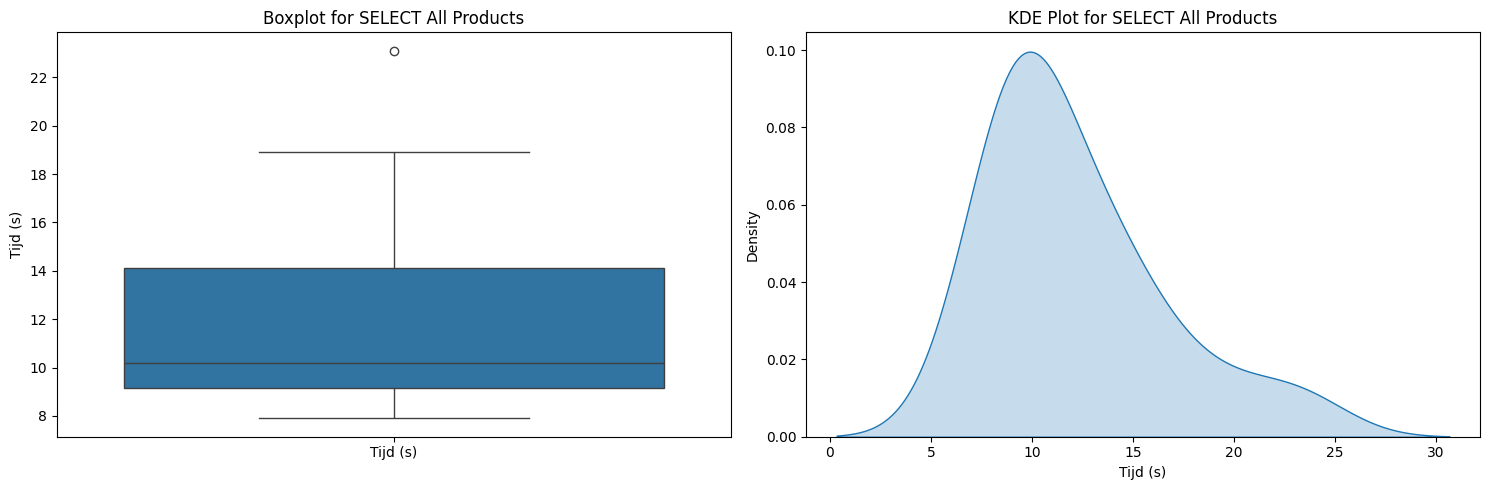
\includegraphics[width=\linewidth]{graphics/couchbase-select}
    \caption[Box- en KDE-plot select all Couchbase]{Box- en KDE-plot voor het selecteren van alle producten in Couchbase}
    \label{fig:couchbase-select}
\end{figure}


\begin{table}[htbp]
    \centering
    \caption{Gemiddelde tijden voor SELECT * FROM fashion.\_default.categories WHERE c8 = 3}
    \begin{tabularx}{\textwidth}{*{8}{>{\centering\arraybackslash}X}c}
        \toprule
        \multicolumn{8}{c}{Tijd (s)} & Gemiddelde \\
        \midrule
        7.0 & 7.8 & 9.7 & 7.7 & 8.6 & 13.0 & 10.8 & 8.3 & 8.8 \\
        7.9 & 7.9 & 8.5 & 9.9 & 9.7 & 11.2 & 6.5 & & \\
        \bottomrule
    \end{tabularx}
\end{table}

\begin{figure}[H]
    \centering
    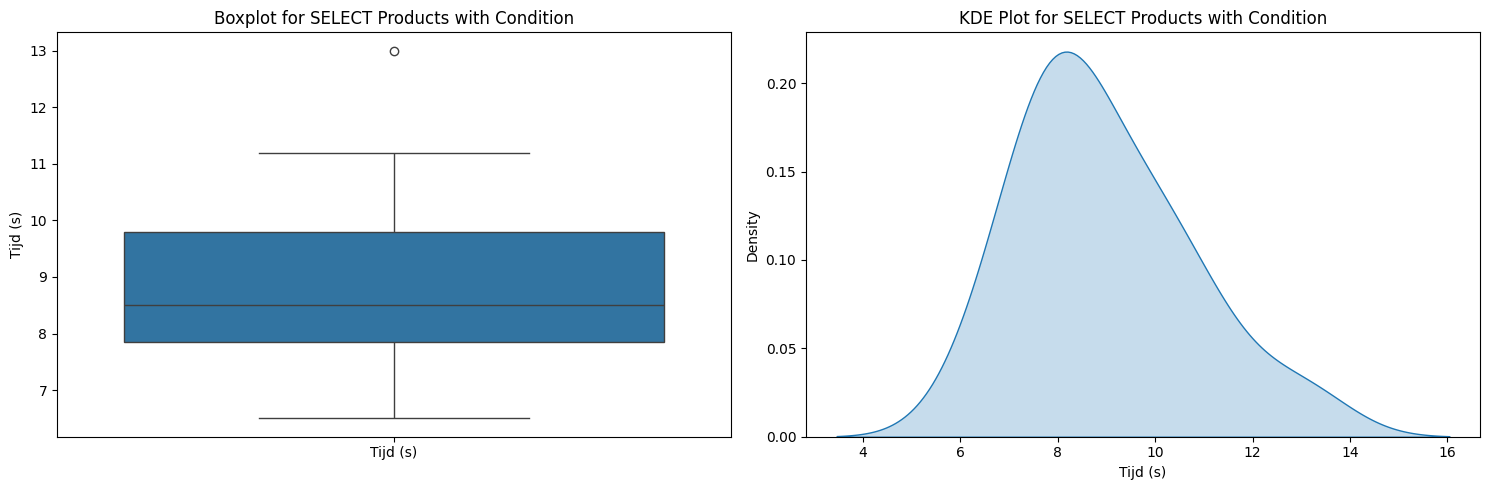
\includegraphics[width=\linewidth]{graphics/couchbase-select-where}
    \caption[Box- en KDE-plot select all where Couchbase]{Box- en KDE-plot voor het selecteren van alle producten die voldoen aan een bepaalde categorie id in Couchbase}
    \label{fig:couchbase-select-where}
\end{figure}


\begin{table}[htbp]
    \centering
    \caption{Gemiddelde tijden voor INSERT INTO categories}
    \begin{tabularx}{\textwidth}{*{8}{>{\centering\arraybackslash}X}c}
        \toprule
        \multicolumn{8}{c}{Tijd (s)} & Gemiddelde \\
        \midrule
        0.0017 & 0.0017 & 0.0014 & 0.0017 & 0.0016 & 0.0020 & 0.0020 & 0.0017 & 0.0017 \\
        0.0018 & 0.0017 & 0.0018 & 0.0018 & 0.0020 & 0.0016 & & \\
        \bottomrule
    \end{tabularx}
\end{table}

\begin{figure}[H]
    \centering
    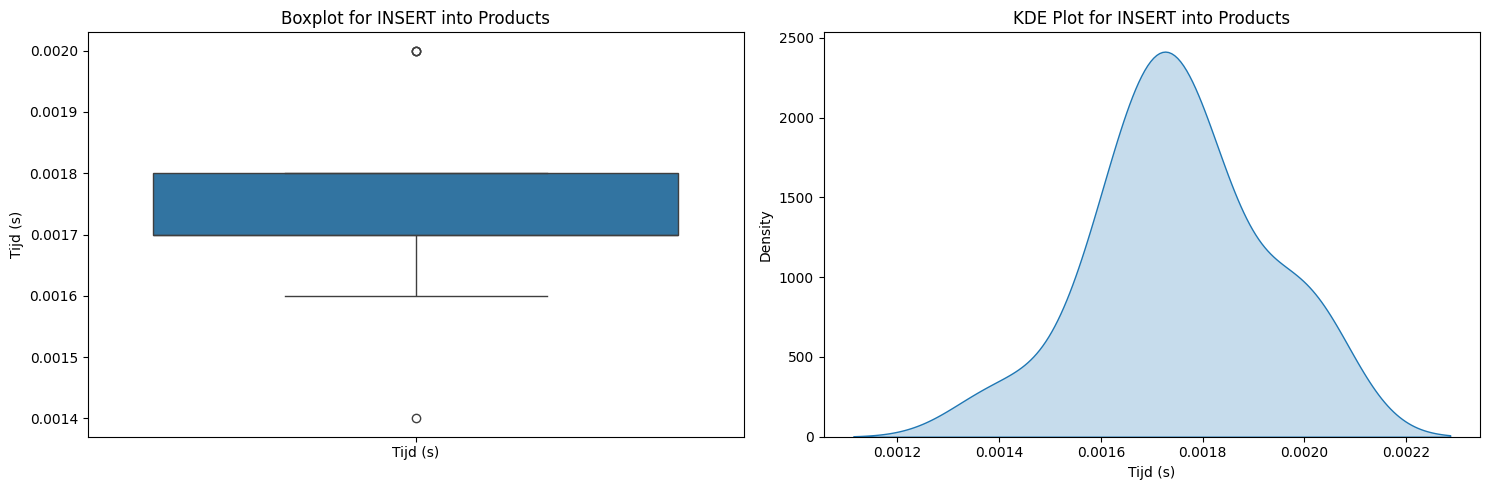
\includegraphics[width=\linewidth]{graphics/couchbase-insert}
    \caption[Box- en KDE-plot insert Couchbase]{Box- en KDE-plot voor het toevoegen van een product in Couchbase}
    \label{fig:couchbase-insert}
\end{figure}


\begin{table}[htbp]
    \centering
    \caption{Gemiddelde tijden voor UPDATE categories}
    \begin{tabularx}{\textwidth}{*{8}{>{\centering\arraybackslash}X}c}
        \toprule
        \multicolumn{8}{c}{Tijd (s)} & Gemiddelde \\
        \midrule
        0.0027 & 0.0024 & 0.0044 & 0.0030 & 0.0025 & 0.0022 & 0.0025 & 0.0026 & 0.0027 \\
        0.0021 & 0.0021 & 0.0026 & 0.0021 & 0.0023 & 0.0021 & & \\
        \bottomrule
    \end{tabularx}
\end{table}

\begin{figure}[H]
    \centering
    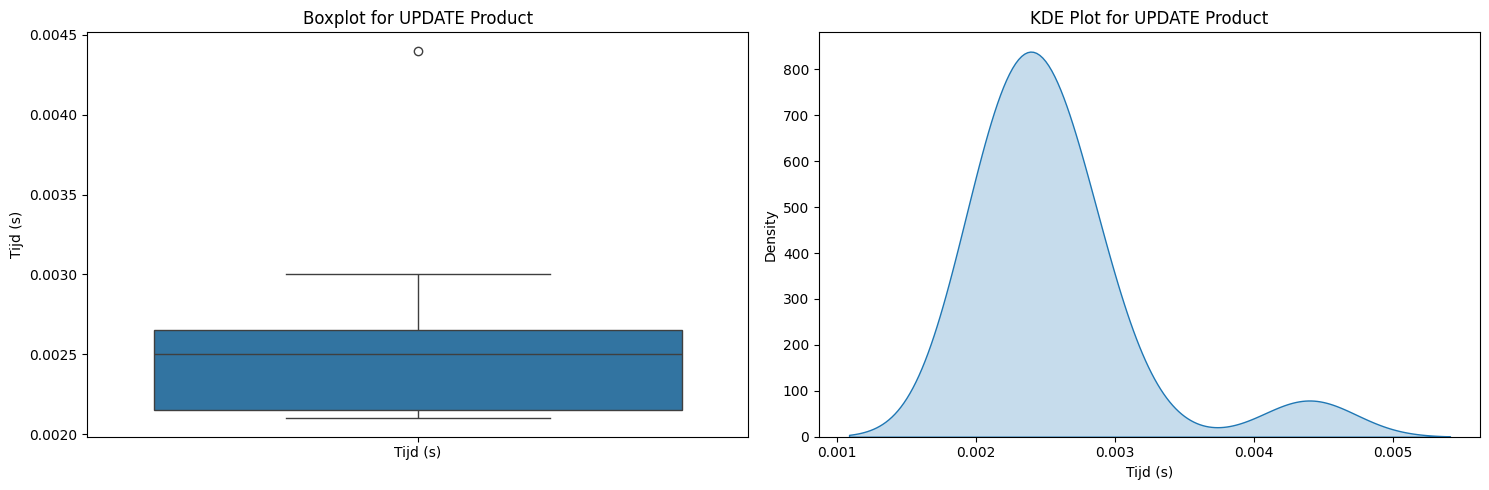
\includegraphics[width=\linewidth]{graphics/couchbase-update}
    \caption[Box- en KDE-plot update Couchbase]{Box- en KDE-plot voor het verhogen van een waarde van een product in Couchbase}
    \label{fig:couchbase-update}
\end{figure}

\begin{table}[htbp]
    \centering
    \caption{Gemiddelde tijden voor DELETE FROM categories}
    \begin{tabularx}{\textwidth}{*{8}{>{\centering\arraybackslash}X}c}
        \toprule
        \multicolumn{8}{c}{Tijd (s)} & Gemiddelde \\
        \midrule
        0.0044 & 0.0017 & 0.0017 & 0.0018 & 0.0018 & 0.0017 & 0.0018 & 0.0018 & 0.0021 \\
        0.0017 & 0.0018 & 0.0014 & 0.0022 & 0.0018 & 0.0017 & & \\
        \bottomrule
    \end{tabularx}
\end{table}

\begin{figure}[H]
    \centering
    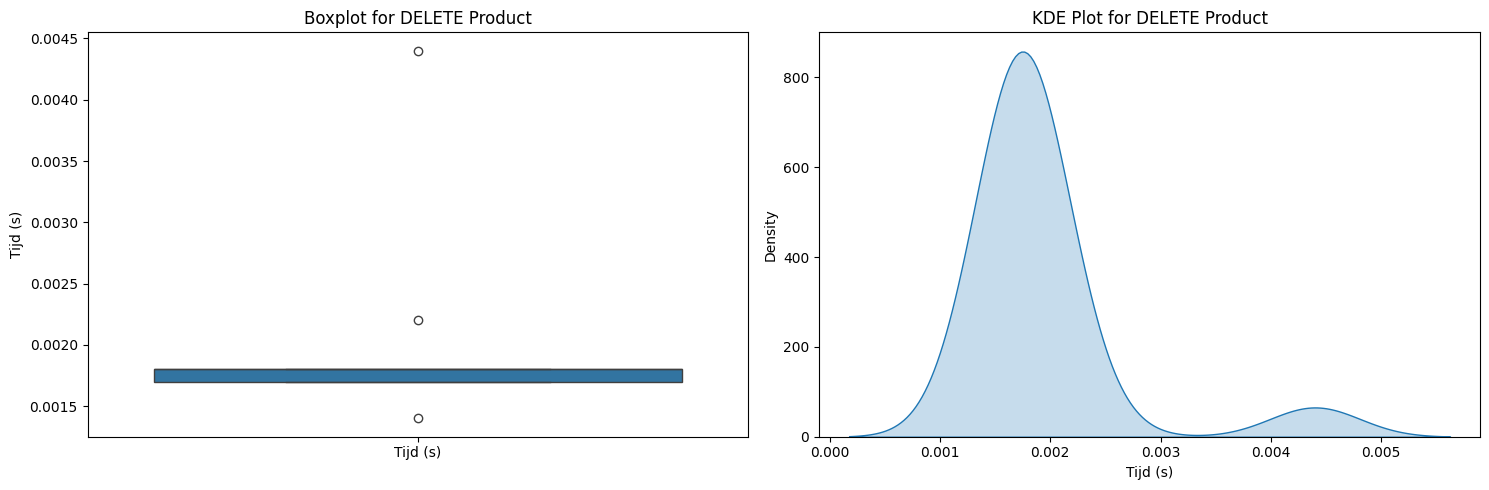
\includegraphics[width=\linewidth]{graphics/couchbase-delete}
    \caption[Box- en KDE-plot delete Couchbase]{Box- en KDE-plot voor het verwijderen van een product in Couchbase}
    \label{fig:couchbase-delete}
\end{figure}


\newpage

\section{\IfLanguageName{dutch}{Amazon Aurora}{Amazon Aurora}}%
\label{sec:test-amazonaurora}

Voor Amazon Aurora zijn er geen technische testen uitgevoerd aangezien voor het opzetten van een database op AWS een creditcard vereist was en deze niet beschikbaar kon gesteld worden. Hierdoor konden de gewenste performance testen en vergelijkingen met andere databases niet worden uitgevoerd.



\section{\IfLanguageName{dutch}{ClickHouse}{ClickHouse}}%
\label{sec:clickhouse}

\subsection{\IfLanguageName{dutch}{Opzetten database}{Creating database}}%
\label{subsec:creating-clickhouse}

Net zoals bij de andere databases, met uitzondering van MariaDB, werd voor het vullen van de ClickHouse-database een CSV-bestand gebruikt met eerder verzamelde data. ($\pm$ 1.9 miljoen rijen) Voor het uitvoeren van de queries is gebruik gemaakt van de Command Line Interface (CLI) die ClickHouse ter beschikking stelt. Dit zorgt ervoor dat nauwkeurige gegevens over de uitgevoerde queries makkelijk kunnen worden verzameld en geanalyseerd.

\begin{figure}[H]
    \centering
    \includegraphics[width=\linewidth]{"graphics/ClickHouse Query"}
    \caption[Voorbeeld query ClickHouse]{Voorbeeld query ClickHouse}
    \label{fig:clickhouse-query}
\end{figure}

Figuur \ref{fig:clickhouse-query} toont een screenshot van de ClickHouse CLI waarin een SELECT-query is uitgevoerd. Onder de gevonden resultaten kan meer informatie worden gevonden over de uitgevoerde query, zoals bijvoorbeeld de querysnelheid, het aantal gevonden rijen, en andere relevante details.


\newpage
Hieronder volgen enkele gebruikte queries:

\begin{lstlisting}[language=SQL, caption={Couchbase-queries voor het beheren van producten in de database.}]
    -- Query 1: Select all products
    SELECT * FROM producten;
    
    -- Query 2: Toevoegen van een categorie
    INSERT INTO categories (c1, c2) 
    VALUES ('new_category', 'new_description');
    
    -- Query 3: Updaten van een product
    ALTER TABLE producten 
    UPDATE c5 = toString(toUInt32(c5) + 1) WHERE c1 = '1'
    
    -- Query 4: Verwijderen van een categorie
    DELETE FROM categories 
    WHERE c1 = 'new_category' AND c2 = 'new_description';
\end{lstlisting}


\subsection{\IfLanguageName{dutch}{Resultaten}{Results}}%
\label{subsec:results5}

Na het uitvoeren van de verschillende queries werden voor ClickHouse volgende resultaten verkregen:

% Table for SELECT * FROM producten
\begin{table}[htbp]
    \centering
    \caption{Gemiddelde tijden voor SELECT * FROM producten}
    \begin{tabularx}{\textwidth}{*{8}{>{\centering\arraybackslash}X}c}
        \toprule
        \multicolumn{8}{c}{Tijd (s)} & Gemiddelde \\
        \midrule
        0.307 & 0.243 & 0.243 & 0.240 & 0.277 & 0.250 & 0.255 & 0.236 & 0.261 \\
        0.243 & 0.264 & 0.263 & 0.235 & 0.282 & 0.253 & 0.293 & & \\
        \bottomrule
    \end{tabularx}
\end{table}

\begin{figure}[H]
    \centering
    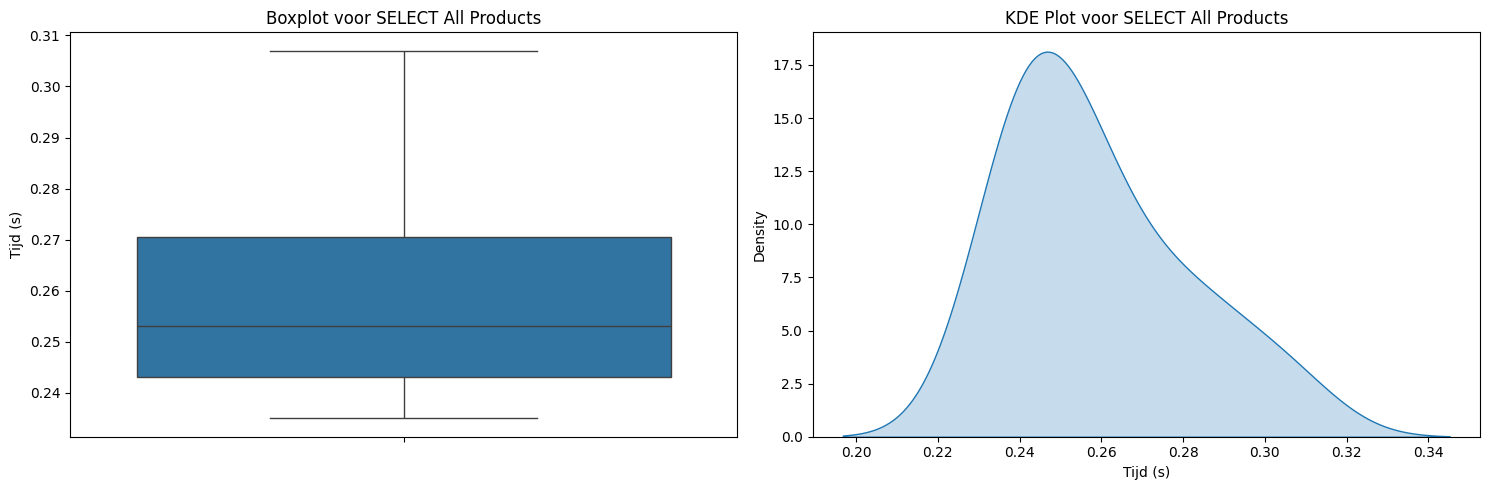
\includegraphics[width=\linewidth]{graphics/clickhouse-all}
    \caption[Box- en KDE-plot select all ClickHouse]{Box- en KDE-plot voor het selecteren van alle producten in ClickHouse}
    \label{fig:clickhouse-all}
\end{figure}


% Table for SELECT * FROM producten INNER JOIN categories
\begin{table}[htbp]
    \centering
    \caption{Gemiddelde tijden voor SELECT * FROM producten INNER JOIN categories}
    \begin{tabularx}{\textwidth}{*{8}{>{\centering\arraybackslash}X}c}
        \toprule
        \multicolumn{8}{c}{Tijd (s)} & Gemiddelde \\
        \midrule
        0.383 & 0.365 & 0.391 & 0.466 & 0.411 & 0.432 & 0.389 & 0.379 & 0.397 \\
        0.367 & 0.434 & 0.423 & 0.382 & 0.424 & 0.340 & 0.362 & & \\
        \bottomrule
    \end{tabularx}
\end{table}
\begin{figure}[H]
    \centering
    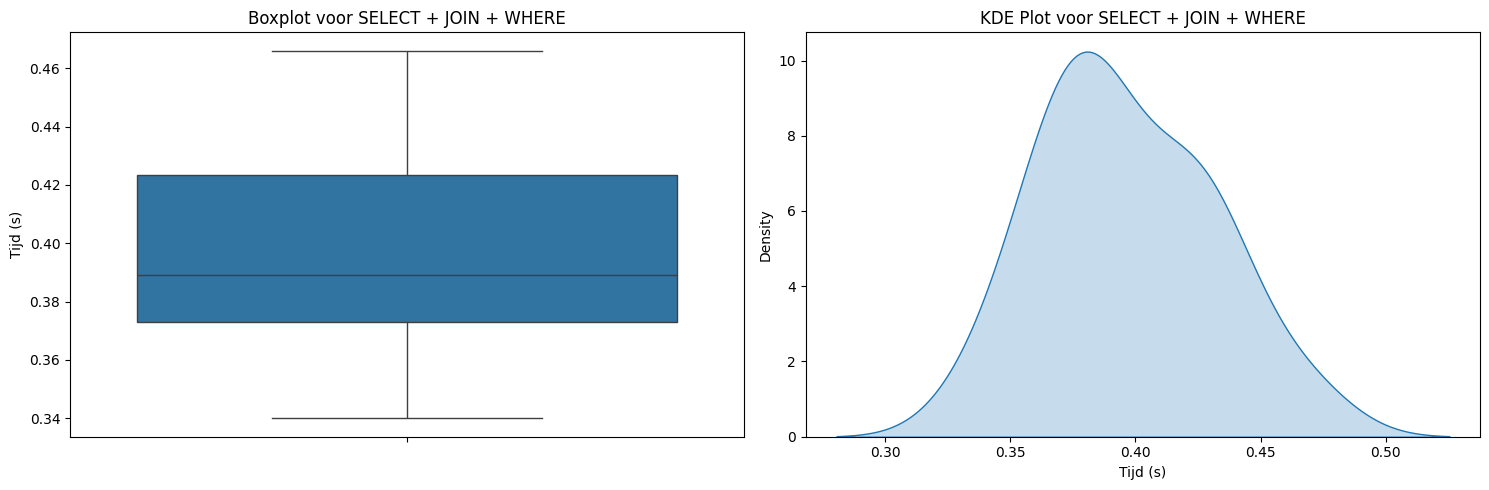
\includegraphics[width=\linewidth]{graphics/clickhouse-all-where}
    \caption[Box- en KDE-plot select all where ClickHouse]{Box- en KDE-plot voor het selecteren van alle producten die voldoen aan een bepaalde categorie id in ClickHouse}
    \label{fig:clickhouse-all-where}
\end{figure}

% Table for INSERT INTO producten
\begin{table}[htbp]
    \centering
    \caption{Gemiddelde tijden voor INSERT INTO producten}
    \begin{tabularx}{\textwidth}{*{8}{>{\centering\arraybackslash}X}c}
        \toprule
        \multicolumn{8}{c}{Tijd (s)} & Gemiddelde \\
        \midrule
        0.065 & 0.072 & 0.060 & 0.081 & 0.095 & 0.071 & 0.098 & 0.078 & 0.078 \\
        0.074 & 0.072 & 0.086 & 0.082 & 0.096 & 0.101 & 0.065 & & \\
        \bottomrule
    \end{tabularx}
\end{table}

\begin{figure}[H]
    \centering
    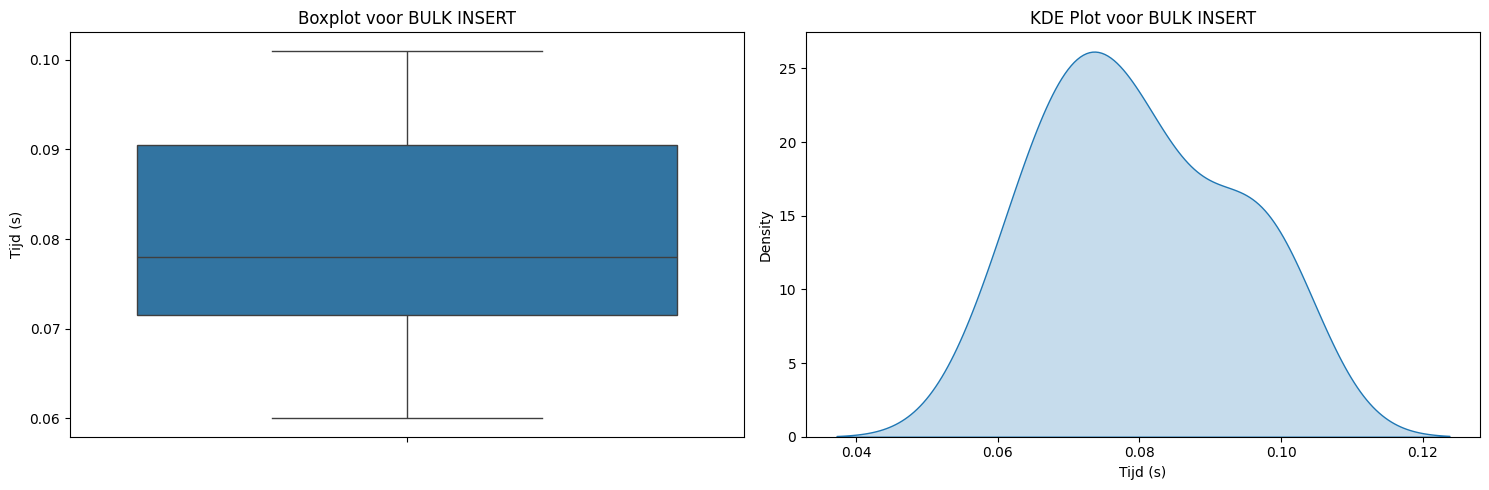
\includegraphics[width=\linewidth]{graphics/clickhouse-bulk-insert}
    \caption[Box- en KDE-plot insert ClickHouse]{Box- en KDE-plot voor het toevoegen van een product in ClickHouse}
    \label{fig:clickhouse-bulk-insert}
\end{figure}


% Table for UPDATE producten SET c5
\begin{table}[htbp]
    \centering
    \caption{Gemiddelde tijden voor UPDATE producten SET c5}
    \begin{tabularx}{\textwidth}{*{8}{>{\centering\arraybackslash}X}c}
        \toprule
        \multicolumn{8}{c}{Tijd (s)} & Gemiddelde \\
        \midrule
        0.056 & 0.059 & 0.058 & 0.057 & 0.054 & 0.054 & 0.055 & 0.058 & 0.055 \\
        0.057 & 0.054 & 0.055 & 0.055 & 0.054 & 0.053 & 0.053 & & \\
        \bottomrule
    \end{tabularx}
\end{table}

\begin{figure}[H]
    \centering
    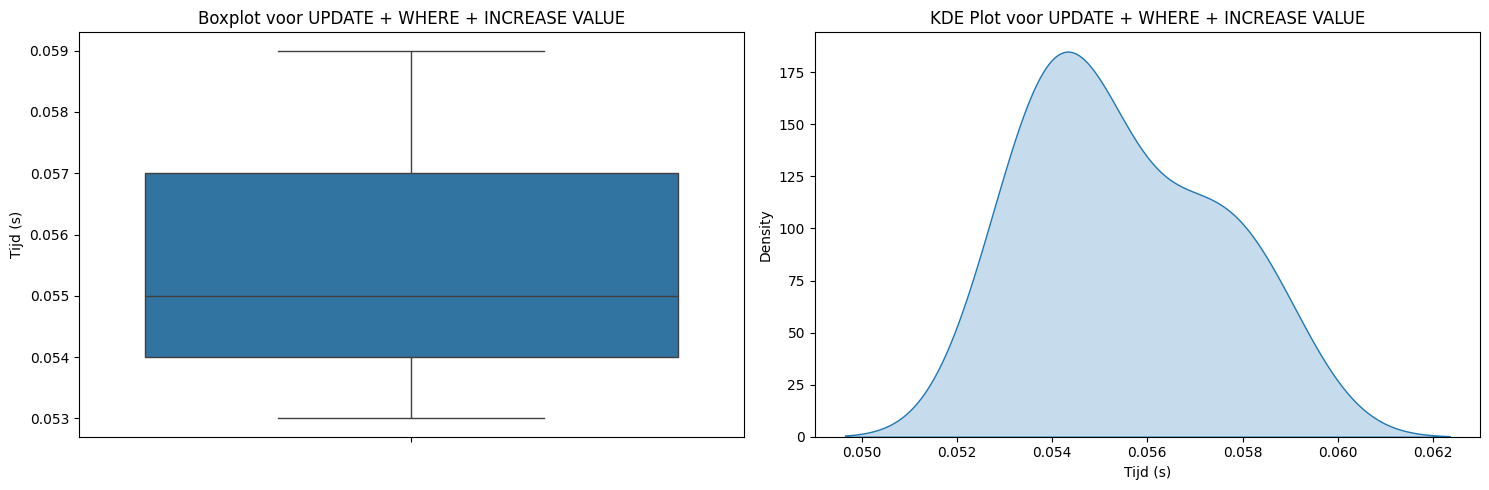
\includegraphics[width=\linewidth]{graphics/clickhouse-update}
    \caption[Box- en KDE-plot update ClickHouse]{Box- en KDE-plot voor het verhogen van een waarde van een product in ClickHouse}
    \label{fig:clickhouse-update}
\end{figure}


% Table for DELETE FROM categories
\begin{table}[htbp]
    \centering
    \caption{Gemiddelde tijden voor DELETE FROM categories}
    \begin{tabularx}{\textwidth}{*{8}{>{\centering\arraybackslash}X}c}
        \toprule
        \multicolumn{8}{c}{Tijd (s)} & Gemiddelde \\
        \midrule
        0.126 & 0.125 & 0.128 & 0.151 & 0.130 & 0.131 & 0.117 & 0.128 & 0.129 \\
        0.130 & 0.132 & 0.129 & 0.135 & 0.120 & 0.143 & 0.130 & & \\
        \bottomrule
    \end{tabularx}
\end{table}

\begin{figure}[H]
    \centering
    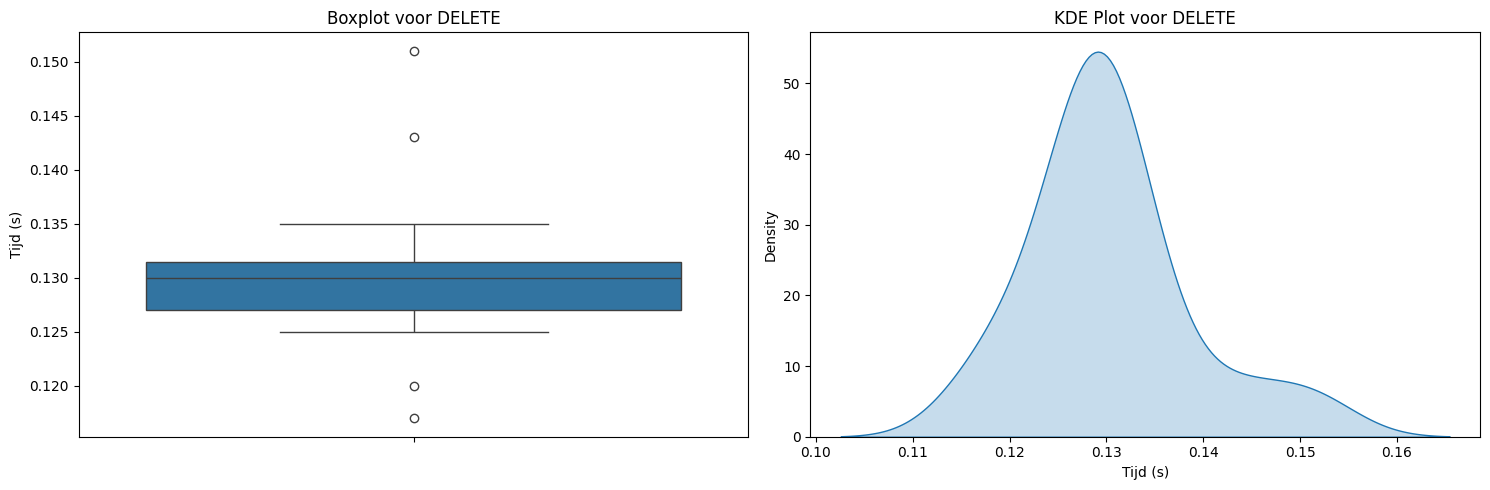
\includegraphics[width=\linewidth]{graphics/clickhouse-delete}
    \caption[Box- en KDE-plot delete ClickHouse]{Box- en KDE-plot voor het verwijderen van een product in ClickHouse}
    \label{fig:clickhouse-delete}
\end{figure}



\newpage


\section{\IfLanguageName{dutch}{Conclusie}{Conclusie}}%
\label{sec:test-conclusie}

Aan de hand van de verzamelde resultaten van MariaDB, MongoDB, Couchbase en Clickhouse kunnen de prestaties met elkaar vergeleken worden. De gemiddelde tijden voor elke uitgevoerde operatie geven een beter inzicht in de efficiëntie en snelheid van elk van deze databases. Het is echter belangrijk om te vermelden dat niet alle resultaten 100\% betrouwbaar zijn. Veel van de uitgevoerde queries werden uitgevoerd in de cloud. Dit zorgt ervoor dat verschillende factoren zoals bijvoorbeeld netwerkvertragingen en serverbelasting de resultaten kunnen beïnvloeden. Daarnaast werd ook niet evenveel data gebruikt voor elk van deze databases vanwege de beperkingen die werden opgelegd door de free trials. Bovendien kon de Amazon Aurora database niet getest worden wegens het ontbreken van een creditcard voor het opzetten van deze database. Ondanks de hierboven beschreven beperkingen worden hieronder de belangrijkste conclusies uit de resultaten weergegeven.

\vspace{5mm}

Wat betreft het ophalen van gegevens blijkt uit de resultaten dat ClickHouse de beste prestaties biedt met een respectief gemiddelde van 0.261 en 0.397 seconden. Daarna komen MongoDB met 0.964 en 1.353 seconden en MariaDB met 4.479 en 4.836 seconden. Couchbase scoorde het slechtst met een gemiddelde van maar liefst 11.8 en 8.8 seconden. Het is nogmaals belangrijk om te melden dat MariaDB de meeste data gebruikt heeft voor deze metingen. Uit deze gemiddelde berekeningen kan besloten worden dat hoewel meer data gebruikt was voor de MariaDB database, ClickHouse mogelijks de betere database is voor het ophalen van grote hoeveelheden aan gegevens. 

\vspace{5mm}

Een database moet echter meer doen dan enkel gegevens ophalen. Ze moeten ook in staat zijn om snel gegevens op te slaan, te verwijderen en bij te werken. Voor het toevoegen van gegevens scoort Couchbase het best.

Ook voor het verwijderen van gegevens heeft Couchbase de beste resultaten. Na Couchbase volgen MariaDB, MongoDB en ClickHouse in hun respectievelijke volgorde.

Voor het updaten van de gegevens scoort MariaDB het slechts met een gemiddelde tijd van 11.865 seconden. Dit is aanzienlijk meer dan de gemiddelde tijden van zowel Couchbase, ClickHouse en MongoDB. OOk hier scoort Couchbase het best. 

\vspace{5mm}

Het is echter belangrijk om te benadrukken dat de betrouwbaarheid van deze resultaten beïnvloed kan zijn door verschillende factoren in de cloudomgeving, zoals:
\begin{itemize}
    \item \textbf{Netwerkvertragingen}: Variaties in de netwerk latency kunnen de responstijden beïnvloeden.
    \item \textbf{Serverbelasting}: De belasting op de servers tijdens het uitvoeren van de queries kan de prestaties beïnvloeden.
    \item \textbf{Resourcebeschikbaarheid}: Fluctuaties in de beschikbaarheid van CPU, geheugen en opslag kunnen de prestaties variëren.
    \item \textbf{Geografische locatie van de servers}: Afstanden tussen de servers en de clients kunnen de netwerkvertragingen verhogen.
\end{itemize}

\vspace{5mm}

Op basis van de gevonden resultaten en rekening houdende met de verschillende factoren kan besloten worden dat voor het uitvoeren van lees-intensieve operaties (SELECT) Clickhouse de beste prestaties biedt. Voor schrijf-intensieve operaties (INSERT en UPDATE) presteert Couchbase zeer goed, hoewel MariaDB en Clickhouse ook competitief zijn. MariaDB blinkt uit bij BULK INSERT operaties. Over het algemeen lijkt Clickhouse de beste oplossing voor een e-commerce webshop in de mode-industrie. Het is belangrijk om de genoemde factoren in de cloudomgeving mee in overweging te nemen bij het interpreteren van deze resultaten.



% Voeg hier je eigen hoofdstukken toe die de ``corpus'' van je bachelorproef
% vormen. De structuur en titels hangen af van je eigen onderzoek. Je kan bv.
% elke fase in je onderzoek in een apart hoofdstuk bespreken.

%\input{...}
%\input{...}
%...

%%=============================================================================
%% Conclusie
%%=============================================================================

\chapter{Conclusie}%
\label{ch:conclusie}

% TODO: Trek een duidelijke conclusie, in de vorm van een antwoord op de
% onderzoeksvra(a)g(en). Wat was jouw bijdrage aan het onderzoeksdomein en
% hoe biedt dit meerwaarde aan het vakgebied/doelgroep? 
% Reflecteer kritisch over het resultaat. In Engelse teksten wordt deze sectie
% ``Discussion'' genoemd. Had je deze uitkomst verwacht? Zijn er zaken die nog
% niet duidelijk zijn?
% Heeft het onderzoek geleid tot nieuwe vragen die uitnodigen tot verder 
%onderzoek?

\lipsum[76-80]



%---------- Bijlagen -----------------------------------------------------------

\appendix

\chapter{Onderzoeksvoorstel}

Het onderwerp van deze bachelorproef is gebaseerd op een onderzoeksvoorstel dat vooraf werd beoordeeld door de promotor. Dat voorstel is opgenomen in deze bijlage.

%% TODO: 
%\section*{Samenvatting}

% Kopieer en plak hier de samenvatting (abstract) van je onderzoeksvoorstel.

% Verwijzing naar het bestand met de inhoud van het onderzoeksvoorstel
%---------- Inleiding ---------------------------------------------------------

\section{Introductie}%
\label{sec:introductie}

De keuze van de juiste databaseoplossing is van belang voor het succes van online mode-e-commerce platformen. Dit onderzoek is gericht op het identificeren van een databasearchitectuur die een balans biedt tussen prestaties en kostenbeheersing voor kleine tot middelgrote mode-e-commerce platformen. Gedurende een periode van vier maanden zullen verschillende databasebeheersystemen geëvalueerd worden op basis van de reactietijd, doorvoersnelheid en operationele kosten. Het einddoel van dit onderzoek is om een gestructureerde benadering te realiseren die mode-ondernemers kan helpen bij het maken van beslissingen op basis van data voor hun e-commerce systemen. De resultaten zullen een duidelijker beeld geven over hoe kleinere e-commerce ondernemingen zich kunnen schalen en klanttevredenheid kunnen verbeteren door de selectie van de gepaste technologieën. Hiermee wordt ook meteen volgende onderzoeksvraag opgelost: ``Hoe evalueren verschillende databaseoplossingen op het gebied van prestaties en kosten voor het ondersteunen van een kleine e-commerce website in de mode-industrie, binnen een onderzoeksperiode van vier maanden?''.

%---------- Stand van zaken ---------------------------------------------------

\section{Literatuurstudie}%
\label{sec:literatuurstudie}
In deze studie wordt, binnen een onderzoeksperiode van vier maanden, nagegaan welke
verschillende databaseoplossingen het meest geschikt zijn op gebied van prestaties en kosten voor
het ondersteunen van kleine e-commerce websites in de mode-industrie. Het onderzoek richt zich op
het identificeren van de meest geschikte databasesystemen die zowel efficiënt als kosteneffectief
zijn voor kleinere ondernemingen in de snel veranderende modebranche.

Voor het opbouwen van een succesvol e-commerce platform in de modebranche is het kiezen van
een concrete databaseoplossing van cruciaal belang. Tegenwoordig is het maken van die keuze
echter niet meer vanzelfsprekend. Bij het maken van een keuze moet er rekening gehouden worden
met verschillende belangrijke factoren, zoals bijvoorbeeld de kosten die deze oplossing met zich
meebrengt, de betrouwbaarheid van de database, de schaalbaarheid en de prestaties. Voor het
bouwen van een moderne e-commerce website, en meer specifiek één in de mode-industrie is er
vooral nood aan een databaseoplossing waarbij er snel en efficiënt omgegaan kan worden met grote
hoeveelheden aan ongestructureerde data en dit terwijl er een optimale gebruikerservaring
behouden wordt. Hiernaast is het ook belangrijk dat deze oplossing kosteneffectief is zodat kleine
bedrijven geen last ondervinden van te hoge operationele kosten.

De populaire NoSQL-database, MongoDB, die bekend staat voor zijn vermogen om flexibel om te
gaan met ongestructureerde data is daarom mogelijks een interessante keuze voor dynamische en
data-intensieve e-commerce platforms~\autocite{Inetum2022}. MongoDB's document-
georiënteerde benadering maakt het geschikt voor toepassingen die snelle ontwikkeling vereisen en
daarbovenop levert het goede resultaten in het omgaan met grote volumes aan diverse data. Echter,
kunnen de kosten voor het gebruik van MongoDB variëren, afhankelijk van de schaal en de vereiste
functionaliteiten, wat een aandachtspunt is voor kostengevoelige projecten.

Anderzijds is er ook de mogelijkheid om gebruik te maken van een traditionele SQL-database, zoals
MySQL of PostgreSQL. Deze databases staan bekend om hun robuustheid bij het verwerken van
gestructureerde gegevens en hun complexe zoekopdrachten. Volgens \textcite{Solarwinds} zijn traditionele databases met name geschikt voor het uitvoeren van transactie-intensieve applicaties,
zoals die vaak voorkomen in e-commerceomgevingen. Ze bieden een hoge betrouwbaarheid en sterke consistentie, maar zijn mogelijk minder flexibel in termen van schemawijzigingen. Ze kunnen ook uitdagingen opleveren bij het opschalen naar grote hoeveelheden ongestructureerde gegevens.

Naast traditionele SQL- of NoSQL-databases kan ook gebruik worden gemaakt van een Graph-database. Zowel ~\textcite{AWS} als ~\textcite{Foote2023} benadrukken dat Graph-databases een flexibeler platform bieden voor het detecteren en tot stand brengen van verbindingen en relaties. Door hun ontwerp zijn grafische databases vaak ook sneller in het presenteren van relaties dan relationele databases. Volgens ~\textcite{AWS} biedt een grafische database echter alleen meerwaarde voor datasets met sterke onderlinge verbindingen en de daarbij behorende analyses, waarbij verborgen en schijnbare relaties moeten worden onthuld.

Een mogelijke oplossing om zowel flexibel om te kunnen gaan met ongestructureerde data als
gestructureerde transactiedata is door gebruik te maken van een hybride benadering ~\autocite{DevX2023}. Dit laat toe om
gebruik te maken van een NoSQL database voor het beheer van dynamische, ongestructureerde
data, zoals MongoDB, en het gebruik van een SQL-database voor de gestructureerde transactiedata
zoals MySQL of PostgreSQL. Hierdoor zouden niet alleen de prestaties worden geoptimaliseerd maar
zouden ook de kosten beheerst kunnen worden. Dit is essentieel voor kleine bedrijven in een
competitieve markt.

Het uiteindelijke doel bestaat erin om een databaseoplossing te vinden die een optimale balans biedt
tussen de kosten en prestaties enerzijds en de flexibiliteit waarmee ingespeeld kan worden op de
veranderende behoeften van de mode-industrie anderzijds.

% Voor literatuurverwijzingen zijn er twee belangrijke commando's:
% \autocite{KEY} => (Auteur, jaartal) Gebruik dit als de naam van de auteur
%   geen onderdeel is van de zin.
% \textcite{KEY} => Auteur (jaartal)  Gebruik dit als de auteursnaam wel een
%   functie heeft in de zin (bv. ``Uit onderzoek door Doll & Hill (1954) bleek
%   ...'')



%---------- Methodologie ------------------------------------------------------
\section{Methodologie}
\label{sec:methodologie}

\subsection{Fase 1: Literatuurstudie}
\label{subsec:literatuurstudie}
In de eerste fase zal er een uitgebreide literatuurstudie uitgevoerd worden om de huidige stand van zaken in database technologieën voor e-commerce platformen in kaart te brengen. Er zullen relevante academische papers, technische documentatie, en marktanalyses bestudeerd worden. Deze fase zal tussen de drie en vier weken duren.
\textbf{Deliverables:} Een overzicht van bestaande databaseoplossingen en een samenvatting van relevante onderzoeksartikelen.

\subsection{Fase 2: Requirements-analyse}
\label{subsec:requirementsanalyse}
In de tweede fase zal er onderzocht worden wat de functionele en niet-functionele eisen zijn voor kleine tot middelgrote mode-e-commerce platformen. Dit zal gedaan worden door in gesprek te gaan of het sturen van mails met stakeholders in kleine tot middelgrote mode-e-commerce platformen. Deze fase zal ongeveer één à twee weken duren.

\textbf{Deliverables:} Een lijst van requirements voor de databasearchitectuur.

\subsection{Fase 3: Experimenteel Ontwerp}
\label{subsec:experimenteelontwerp}
In deze fase zal een reeks experimenten opgezet worden om verschillende databasebeheersystemen te evalueren. Deze experimenten zullen zich richten op prestatie-indicatoren zoals reactietijd en doorvoersnelheid. Deze fase zal ongeveer één à twee weken duren.

\textbf{Deliverables:} Een experimenteel plan en testprotocollen.

\subsection{Fase 4: Data-analyse}
\label{subsec:dataanalyse}
In fase vier zal de verzamelde data uit de experimenten geanalyseerd worden met statistische software om significante patronen en verschillen te identificeren. Deze fase zal ongeveer één à twee weken duren.

\textbf{Deliverables:} Een statistisch onderbouwd rapport met de bevindingen uit de experimenten.

\subsection{Fase 5: Vergelijkende Studie}
\label{subsec:vergelijkendestudie}
In de vijfde fase zal op basis van de data-analyse een vergelijkende studie uitgevoerd worden om de voor- en nadelen van elk databasebeheersysteem te identificeren. Deze fase zal ongeveer één tot twee weken duren.

\textbf{Deliverables:} Een gedetailleerde vergelijkingstabel en een aanbevelingsrapport.

\subsection{Fase 6: Risico-analyse}
\label{subsec:risicoanalyse}
In deze fase zal er een risico-analyse uitgevoerd worden om potentiële knelpunten en risico's in de implementatie van de aanbevolen databaseoplossingen te identificeren. Deze fase zal ongeveer een week duren.

\textbf{Deliverables:} Een risicobeoordelingsdocument.

\subsection{Fase 7: Proof of Concept (PoC)}
\label{subsec:poc}
In deze fase zal een Proof of Concept ontwikkeld worden om de haalbaarheid van de aanbevolen databasearchitectuur te demonstreren. Deze fase zal ongeveer een week duren.

\textbf{Deliverables:} Een werkend prototype en een documentatie van de ontwikkeling.

\subsection{Fase 8: Rapportering en documentatie}
\label{subsec:rapporteringendocumentatie}
Tijdens voorlaatste fase zal er een rapport en documentatie gemaakt worden van het hele proces
van het onderzoek. Dit zal gebeuren aan de hand van alle verzamelde informatie tijdens het onderzoek. Aan het einde van deze fase zal de bachelorproef volledig voltooid zijn. Deze fase zal één tot twee weken duren.

\textbf{Deliverables:} Een bijna volledig afgewerkte bachelorproef.

\subsection{Fase 9: Review en afronding}
\label{subsec:reviewenafronding}
In de laatste fase zullen alle documenten herbekeken worden om te zorgen dat alles in orde is. Deze
documenten zullen dan meerde keren gecheckt worden op taalfouten en andere fouten. Wanneer deze fase voltooid is, zal de bachelorproef klaar zijn om ingediend te worden en is het onderzoek afgelopen. Deze fase zal ongeveer één à
twee weken duren.

\textbf{Deliverables:} Een volledig afgewerkte bachelorproef.

\begin{figure}[htbp]
    \centering
    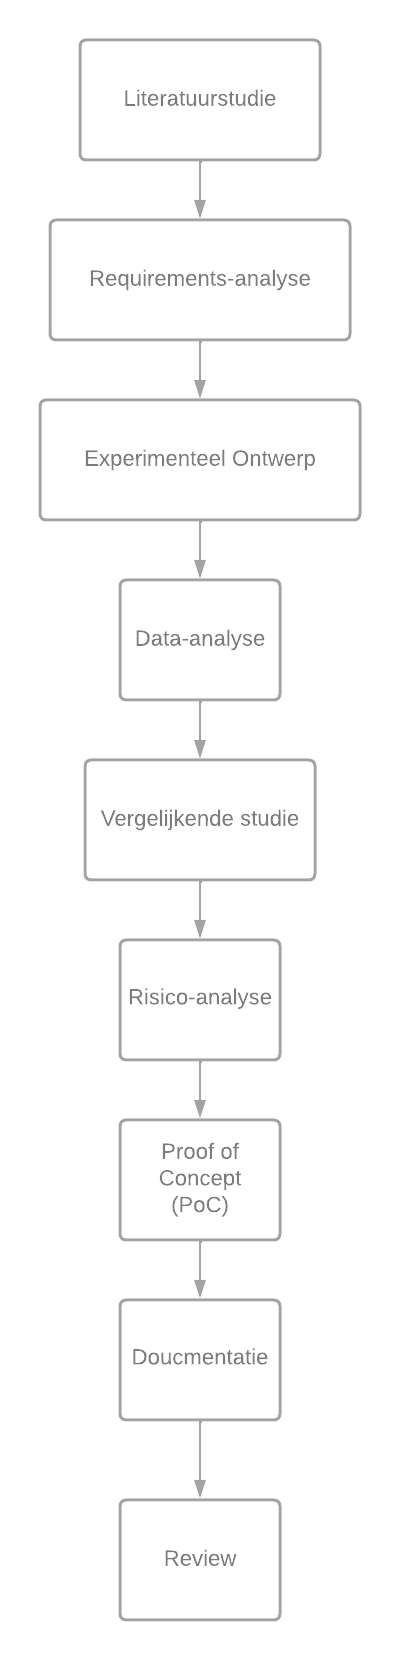
\includegraphics[width=0.3\textwidth]{Flowchart.png}
    \caption{Flowchart van het onderzoeksproces.}
    \label{fig:flowchart}
\end{figure}


%---------- Verwachte resultaten ----------------------------------------------
\section{Verwacht Resultaat en Conclusie}%
\label{sec:verwachte_resultaten}

De verworven kennis geeft momenteel aan dat de ontwikkeling van een hybride systeem, dat
MongoDB als NoSQL-database combineert met MySQL of PostgreSQL, de meest veelbelovende
benadering lijkt in termen van efficiëntie en kostenbeheersing voor kleine en middelgrote mode-e-
commerce platforms. Er wordt verwacht dat vervolgonderzoek diepere inzichten zal verschaffen die
van cruciaal belang zijn bij de keuze van het meest adequate databasemanagementsysteem. Dit
vervolgonderzoek zal de technische specificaties en operationele kostenfactoren grondig moeten
afwegen om een weloverwogen besluit te kunnen nemen.


%---------- References ----------------------------------------------



%%---------- Andere bijlagen --------------------------------------------------
% TODO: Voeg hier eventuele andere bijlagen toe. Bv. als je deze BP voor de
% tweede keer indient, een overzicht van de verbeteringen t.o.v. het origineel.
%\input{...}

%%---------- Backmatter, referentielijst ---------------------------------------

\backmatter{}

\setlength\bibitemsep{2pt} %% Add Some space between the bibliograpy entries
\printbibliography[heading=bibintoc]

\end{document}
